\chapter{Классификация гамма-всплесков, зарегистрированных в эксперименте Конус-Винд}

\section{Введение}
Феноменологическая классификация  гамма-всплесков основана на параметрах 
временной истории в гамма-диапазоне: жесткости, длительности и спектральной задержке. 

Длительность всплесков демонстрирует явное бимодальное 
распределение~\citep{Mazets_1981_part_1,Norris_1984,Kouveliotou_1993,Aptekar_1998}. 
В работе \citep{Kouveliotou_1993} были введены две меры длительности $T_{50}$ и $T_{90}$, 
которые соответствуют временам накопления 50\% и 90\% от суммарного числа отсчётов 
всплеска и определена граница между длинными и короткими всплесками $T_{90}=2$~с 
на основе локального минимума бимодального распределения. 

Систематические ошибки величин $T_{50}$ и $T_{90}$ на примере всплесков, 
зарегистрированных в эксперименте \textit{CGRO}-BATSE~\citep{Fishman_1994}, 
были рассмотрены в работе~\citep{Norris_and_Bonnel_2006}. Было показано, 
что как минимум четыре фактора влияют на измеренное значение длительности 
всплеска и размывают границы между классами длинных и коротких всплесков. 
Различие в отношении сигнал-шум (S/N) между самым интенсивным и самым слабым 
всплеском  при условии, что эти всплески не отличаются по другим параметрам, 
приводит к различию их длительностей $T_{90}$ в $\sim2$~раза \citep{Bonnell_1997}. 
Длительность удалённых длинных всплесков ($z\sim2$--10)  масштабируется в 2--5 раз 
по сравнению со всплесками, пришедшими с $z=1$. В это же время поправка длительности 
для коротких всплесков не превышает двух раз, так как их источники в основном 
расположены на $z<1$. Этот фактор увеличивает обособленность распределений 
коротких и длинных всплесков. Эффект зависимости длительности отдельных импульсов 
всплесков от энергии $\sim E^{-0.35}$ \citep{Fenimore_1995}, а так же  модификация 
спектра за счёт космологического расширения приводит к зависимости длительности 
всплеска от энергетического диапазона наблюдений. Распределение по длительностям 
обрезано со стороны коротких всплесков вследствие наблюдательной селекции триггерного 
алгоритма. 

Кроме $T_{50}$ и $T_{90}$ была предложена и другая мера длительности~--- время 
эмиссии~\citep{Mitrofanov_1999}, которая вычисляется как суммарная длительность 
бинов временной истории, в которых интенсивность излучения превышает заданный 
уровень от пиковой интенсивности. Этот уровень задается таким образом, чтобы 
суммарное число отсчетов в бинах составляло заданную долю от общего числа отсчётов 
всплеска (использовались уровни 30\% и 50\%, соответствующие меры длительности 
были обозначены $\tau_{30}$ и $\tau_{50}$). Было показано, что данная мера 
длительности гораздо менее чувствительна и к отношению сигнал-шум и к количеству 
импульсов во всплеске, разделенных значительным промежутком фона, так как этот 
промежуток не входит по определению в определяемое время эмиссии. Ясно, однако, 
что эта мера чувствительна к временному разрешению. Распределения всплесков 
по $\tau_{30}$ и $\tau_{50}$  также являются бимодальными. Классификация всплесков 
с использованием этой меры длительности в нашей работе не рассматривается. 

В работе \citep{McBreen_1994} обсуждается, что распределение всплесков по 
длительности $T_{90}$ хорошо описывается суммой двух логнормальных компонент. 
На основе данных из третьего каталога эксперимента \textit{CGRO}-BATSE, 
в работе~\citep{Horvath_2002} было показано, что распределение всплесков 
по длительности $T_{90}$ хорошо аппроксимируется тремя логнормальными компонентами. 
Третья компонента располагалась между короткими и длинными всплесками, 
что свидетельствовало о наличие третьего класса всплесков с промежуточной длительностью.

В работе \citep{Kouveliotou_1993}  было обнаружено, что короткие всплески в 
среднем имеют большую жесткость, чем длинные. Жесткость (HR$_{32}$) определялась 
как отношение числа отсчетов, накопленных за $T_{90}$ в энергетических 
диапазонах 100--300~кэВ и 50--100~кэВ –- диапазоны 3 и 2 эксперимента \textit{CGRO}-BATSE. 
В последующих работах было отмечено, что жесткость не является обязательной чертой 
коротких всплесков~\citep[см. например][]{Sakamoto_2006_proc, Norris_and_Bonnel_2006}. 

На основе распределения на плоскости жесткость-длительность также был обнаружен 
третий класс всплесков~\citep{Mukherjee_1998, Hakkila_2000}. Анализ влияния 
систематических эффектов на наличие третьего класса всплесков был проведён 
в~\citep{Hakkila_2003}. Авторы показали, что третий класс всплесков не является 
физическим и может являться следствием селекции триггерного алгоритма. Также было 
показано, что сам по себе эффект зависимости длительности от яркости 
всплеска~\citep{Bonnell_1997} не может привести к появлению третьего класса всплесков. 
Однако, в последующей работе~\citep{Horvath_2006} были приведены доводы в пользу 
реальности третьего класса всплесков, и исследовалось количество и значимость 
классов всплесков на основе параметров распределения на плоскости 
$\log T_{90}$--$\log \rmn{HR}_{32}$ для 1956 всплесков, зарегистрированных 
в эксперименте \textit{CGRO}-BATSE. При этом распределение аппроксимировалось 
суммой двумерных нормальных распределений. Было установлено, что распределение 
наилучшим образом описывается тремя компонентами (классами). При этом доля всплесков 
из третьего класса составляет 10--15\%. Также было показано, что поправка набора 
всплесков на селекцию триггерного алгоритма сохраняет прежнее разделение на классы. 
Аналогичный метод был применен к 222-м всплескам \textit{Swift}-BAT~\citep{Horvath_2010}, 
при этом также было обнаружено три класса всплесков. При этом доля промежуточного 
класса всплесков составила~30\%.

Помимо жесткости и длительности, еще одним параметром для классификации всплесков 
может служить спектральная задержка. Этот параметр характеризует запаздывание 
излучения в более мягком диапазоне по отношению к излучению в более жестком диапазоне. 
Значение задержки ($\tau_{\rmn{lag}}$) соответствует положению  максимума 
кросскорреляционной функции временных историй в двух энергетических диапазонах~\citep{Norris_2000}. 
Анализ спектральных задержек коротких всплесков \textit{CGRO}-BATSE и 
\textit{Swift}-BAT показал, что они распределены вблизи нуля с разбросом 
порядка 25~мс \citep{Norris_and_Bonnel_2006, Norris2011}. В то же время длинные 
всплески могут иметь значительные задержки. Идея о том, что различие спектральных 
задержек длинных и коротких всплесков отражает различие физических свойств источников 
всплесков, была выдвинута в~\citep{Gehrels_2006_Nature}.

%Существует несколько моделей, объясняющих появление спектральной задержки. 
%В работе~\citep{Ioka_and_Nakamura_2001} появление задержки объясняется, тем что 
%узкий джет наблюдается под разными углами для разных всплесков. Большая задержка 
%соответствует большему углу наблюдения относительно оси джета. 
%Авторы работы~\citep{Schaefer_2004_lag} считают, что спектральная задержка в 
%каждом импульсе всплеска характеризует время потери энергии излучающими частицами.

Детектирование рентгеновских послесвечений и локализация источников всплесков с 
точностью несколько угловых минут экспериментом \textit{BeppoSAX}~\citep{Boella1997} 
открыло эру многоволновых наблюдений гамма-всплесков. Впервые красное смещение 
родительской галактики длинного всплеска было измерено в 1997~г для GRB~970228. 
Однако, из-за малой интенсивности и быстрого затухания не удавалось детектировать 
послесвечения коротких всплесков. Эксперимент \textit{Swift}~\citep{Gehrels_2004}, 
запущенный в 2005~г, благодаря возможности быстро локализовать источник всплеска 
позволил измерять красные смещения и находить родительские галактики коротких 
гамма-всплесков. Впервые было зарегистрировано рентгеновское послесвечение и обнаружена 
родительская галактика для короткого всплеска GRB~050509B. На декабрь 2013~г красное 
смещение определено для, примерно, 300 гамма-всплесков, из них около 40~--- короткие всплески.

Многоволновые наблюдения гамма-всплесков и определение свойств их родительских галактик, 
таких как морфологический тип, скорость звездообразования, металличность, позволили 
выдвинуть предположения об источниках всплесков. Источником длинных гамма-всплесков 
считается коллапс массивных звёзд. В пользу этого свидетельствует ассоциация части 
близких длинных всплесков со сверхновыми Типа~Ic и расположение источников длинных 
всплесков в галактиках с высокой скоростью звездообразования, преимущественно в 
наиболее ярких их областях с высокой скоростью звездообразования. В наблюдениях 
оптических послесвечений коротких всплесков поставлены глубокие верхние пределы 
на уярчение связанное со сверхновой. Источники коротких всплесков располагаются 
в галактиках с различной скоростью звездообразования и морфологическим 
типом~\citep[см. обзор][]{Berger_2014}. На основе этих наблюдений, в качестве 
источника коротких всплесков предлагается слияние двух компактных объектов: 
двух нейтронных звёзд или нейтронной звезды и чёрной дыры.

В работах~\citep{Zhang_2006, Zhang_2007, Zhang_2009} была введена схема классификации, 
основанная на параметрах послесвечений и родительских галактик гамма-всплесков. 
Авторы предлагают разделять всплески на два типа I и II. Считается, что всплески 
типа I, генерируются при слиянии компактных объектов. Всплески типа II образуются 
при коллапсе молодых массивных звёзд. В работе~\citep{Zhang_2009} было показано, 
что всплески типа II на плоскости жесткость-длительность располагаются в области 
длинных/мягких всплесков, при этом всплески типа I являются коротким и имеют 
умеренную жесткостью. Авторы также отмечают, что всплески типа I обладают 
незначительной спектральной задержкой.

В этой работе мы анализируем временные истории всплесков, зарегистрированных в 
эксперименте Конус-Винд, и классифицируем их на основе длительности, жесткости и 
спектральной задержки. Мы представляем набор коротких всплесков, которые будут 
включены в каталог коротких всплесков Конус-Винд. При этом обсуждается принадлежность 
исследуемых всплесков к типам~I и~II. В разделе~\ref{sec:GRB_sample} приводится 
описание использованного набора всплесков. 
В разделе~\ref{sec:Durations} рассматривается распределение всплесков по длительности 
и предлагается граница между длинными и короткими всплесками на основе 
длительности $T_{50}$, и описывается итоговый набор коротких всплесков. 
В разделе~\ref{sec:Hardness} рассматриваются жесткости всплесков, и производится 
классификация всплесков на основе соотношения жесткость-длительность. 
В разделе~\ref{sec:Lags} анализируются спектральные задержки коротких и длинных всплесков. 
Сравнение классификации на физические типы~I и~II и классификации на основе жесткости, 
длительности и спектральной задержки приведено в разделе~\ref{sec:Phis_Classification}. 
Обобщение и обсуждение наших результатов приведено в разделе~\ref{sec:Conclision}.  

\section{Набор всплесков}\label{sec:GRB_sample}
За период с ноября 1994~г по декабрь 2010~г было зарегистрировано 2008 гамма-всплесков 
в триггером режиме. Среди них 69 всплесков содержат сбои, представляющие собой 
промежутки в данных во время всплеска или значительные флуктуации фона, 
накладывающиеся на всплеск. Для вычисления параметров временных историй используется 
сшивка фоновой и триггерной записи. Длительность всплесков, у которых значительная 
часть события лежит в фоновом бине предшествующем триггерной записи, может быть 
искажена из-за низкого разрешения фоновой записи. Из дальнейшего рассмотрения 
было исключено 105 таких событий. Таким образом, для анализа использовались временные 
истории 1834 гамма-всплеска. 

\section{Длительности}\label{sec:Durations}
Для вычисления длительностей мы использовали сумму временных историй всплеска 
в энергетических диапазонах G2 и G3. Такой выбор обоснован тем, что  пиковая 
энергия $E F_{E}$ спектра~--- $E_{\rmn{p}}$ абсолютного большинства всплесков лежит в 
диапазоне $E_{\rmn{p}}>80$~кэВ и значит отсчёты, соответствующие  основному энерговыделению 
во всплеске, регистрируются в G2 и G3. Фон в диапазонах G2 и G3 стабилен на более 
длительных интервалах времени, чем в G1. Это позволяет с гораздо меньшей вероятностью 
неверно определять начало и конец всплеска из-за флуктуаций фона. Также в диапазон G1 
может попадать начало рентгеновского послесвечения, учёт которого исказит 
длительность начального импульса всплеска.

\subsection{Определение уровня фона}
Для всех всплесков фон аппроксимировался постоянным значением. Максимальным 
интервалом определения фона был выбран [$T_0 - 1000$~с; $T_0 - 250$~с], 
где $T_0$~--- время срабатывания триггера. Значительный отступ от триггерного 
времени связан с тем, что начало некоторых длинных всплесков лежит в предыстории. 
Время $T_0-250$~с соответствует наибольшему отступу начала всплеска от $T_0$.

Для подтверждения постоянства фона проверялась гипотеза о том, что отсчёты на 
интервале имеют гауссово распределение со средним равным среднему числу отсчётов 
$\overline{N}$ и дисперсией равной $\sqrt{\overline{N}}$. Для проверки гипотезы 
использовался критерий Колмогорова-Смирнова с уровнем значимости 0.01~\citep{Press_1992NumRec}. 
Если гипотеза принималась, то фон считался равным вычисленному среднему. 
Если гипотеза отвергалась, то интервал сокращался на одни бин со стороны наиболее 
удалённой от $T_0$ и процедура повторялась. Из всего набора у 1768 всплесков длина 
фонового интервала равна 750~с, только 8 всплесков имеют длину фонового интервала 30--100~c.

Уровни фона в трех диапазонах детекторов S1 и S2 незначительно различаются, что 
связано с различием границ диапазонов в детекторах. Скорости счёта фона на 2010~г 
равны для детектора S1: $\sim$ 1000 отсч~с$^{-1}$ в G1, $\sim$ 350 отсч~с$^{-1}$ в G2, 
$\sim$ 200 отсч~с$^{-1}$ в G3, для детектора S2: $\sim 1080$~отсч~с$^{-1}$ в G1, 
$\sim 390$~отсч~с$^{-1}$ в G2, $\sim160$~отсч~с$^{-1}$ в G3. Ошибки средней 
скорости счета на уровне $1\sigma$ для всех детекторов равны: в G1 
$\sim 1.3$~отсч~с$^{-1}$, в G2 $\sim 0.7$~отсч~с$^{-1}$, в G3 $\sim 0.5$~отсч~с$^{-1}$. 
Начиная с момента начала работы инструмента уровни фона медленно изменялись, 
что связано с изменением границ диапазонов со временем. Для детектора S1 относительное 
изменение фоновой скорости счёта составляет для G1 $\sim 13$\%, G2 $\sim 46$\%, 
G3 $\sim 18$\%. Для детектора S2 относительное изменение составляет для G1 $\sim 9$\%, 
G2 $\sim 41$\%, G3 $\sim 17$\%. В периоды повышенной солнечной активности наблюдались 
сильные кратковременные вариации фона. 

\subsection{Автоматическая процедура определения длительности}
Основной задачей при вычислении любой меры длительности является определение момента 
начала и конца всплеска. В работе~\citep{Koshut_1996}, описывающей методику вычисления 
длительностей $T_{90}$ и $T_{50}$  для второго каталога BATSE, моменты начала и 
конца всплеска $t_{0}$ и $t_{100}$ определялись визуально на основании интеграла 
от временной истории всплеска, $t_{x}$ соответствует времени накопления заданной 
доли $x$ от полного числа отсчётов всплеска. В работе~\citep{Bonnell_1997} использовалась 
автоматическая процедура поиска $t_{0}$ и $t_{100}$, в которой производится поиск 
положительной флуктуации числа отсчетов с вычетом фона со значимостью от $3\sigma$ 
до $6\sigma$ на временных масштабах от 0.5~с до 16~с в диапазоне~$>25$~кэВ. 

Для вычисления длительности всплесков Конус-Винд использовалась автоматическая 
процедура поиска начала и конца всплеска. Поиск производился на интервале от 
$T_0-250$~с до $T_0+230$~с (конца триггерной записи). Для некоторых всплесков 
границы интервала вычисления длительности устанавливались визуально, к примеру, 
это делалось в случае присутствия солнечной вспышки в данных. Для поиска начала 
всплеска производился поиск положительной флуктуации числа отсчетов с вычетом 
фона на заданном уровне значимости. При этом поиск превышения производился на 
интервале с длительностью от временного разрешения конкретного участка записи до 100~с. 
Началом всплеска $t_0$ считается начало интервала, на котором была обнаружена флуктуация, 
если вероятность её случайного обнаружения была меньше пороговой. Времена начала 
интервалов поиска флуктуаций брались последовательно, начиная от $T_0-250$~с. 
Конец всплеска~--- $t_{100}$ определяется аналогичного, при этом поиск вёлся в 
обратном направлении по времени, начиная от $T_0 + 230$~с. Длительности всплесков 
вычислялись для порогов, соответствующих вероятности случайного превышения 
значений $4\sigma$, $5\sigma$ и $6\sigma$ для распределения Гаусса. При этом на 
интервалах, где число отсчётов от фона меньше 20, для вычисления вероятности 
случайного превышения использовалась статистика Пуассона. Значения $T_{90}$ и $T_{50}$ 
и их ошибки определялись методом, описанном в работе~\citep{Koshut_1996}. 

\subsection{Распределения по длительностям}
Для 1834 всплесков Конус-Винд были построены распределения по $T_{90}$ и $T_{50}$ 
для порогов значимости поиска начала и конца всплеска $4\sigma$, $5\sigma$ и $6\sigma$. 

Из-за эффектов селекции число очень коротких всплесков ($T_{50} \leq 100$~мс) и 
число длинных всплесков ($T_{50} > 200$~с) недооценено в нашем наборе. Так же неверно 
считать ошибки числа отсчётов в бине гауссовыми при числе отсчётов $<10$, поэтому 
бины с $\log T_{90} \leq-1.2$ ($T_{90} \leq 0.063$~с) и $\log T_{90} \geq 2.4$ ($T_{90} \geq 251$~с) 
не учитывались при аппроксимации распределения по $T_{90}$,  для аппроксимации 
использовалось 18 бинов. При аппроксимации распределения по $T_{50}$ игнорировались 
бины c $\log T_{50} \leq -1.8$ ($T_{50} \leq 0.016$~с) и  $\log T_{50} \geq 2.0$ 
($T_{50} \geq 100$~с), для аппроксимации использовалось 19 бинов.

Распределения  аппроксимировались методом минимизации $\chi^2$ суммой двух логнормальных распределений
\begin{equation}
f(x) = \sum_{l=1}^{2} A_l f_l(x) \mbox{ ,}
\end{equation}
где
\begin{equation}
f_l(x) = \frac{1}{w_l \sqrt{\pi/2}} \exp\left(\frac{-2(x-x_{cl})^2}{w_l^2}\right) \mbox{ ,}
\end{equation}
где $A_l$ –- площадь под распределением, $w=2\sigma$~--- ширина, $x_{cl}$~--- среднее значение и 
$x=\log T$. При этом число всплесков в бине по модели равно  интегралу от аппроксимирующей функции в границах бина. 

Доверительные интервалы параметров распределения на уровне 68\% вычислялись 
методом Mонте-Карло для 1000 реализаций распределения. При этом значение в каждом 
бине распределения является пуассоновской случайной величиной со средним равным 
числу отсчётов в соответствующем бине исходного распределения. Полученный набор 
значений каждого параметра сортировался по возрастанию. В качестве нижней и верхней 
границы доверительного интервала на уровне 68\% брались значения с индексами 160 и 840, 
соответственно. В качестве значения параметра бралась медиана распределения.

Параметры распределений представлены в таблицах \ref{tab:T90_distr} и~\ref{tab:T50_distr}. 
Из представленных результатов видно, что при изменении порога от $4\sigma$ до $6\sigma$ 
параметры распределения по $T_{50}$ и $T_{90}$ для полного набора 1834 всплесков изменяются. 
Распределение длинных всплесков смещается в сторону меньших длительностей, такое же смещение, 
но в меньшей степени, наблюдается для распределение коротких всплесков. 
При этом изменение параметров распределения по $T_{90}$ гораздо существенней, 
чем для распределения по $T_{50}$: 
$\delta T_{90c1} = 19$\%, $\delta T_{90c2} = 27$\%, $\delta T_{90int} = 14$\%, 
$\delta T_{50c1} = 7$\%, $\delta T_{50c2} = 13$\%, $\delta T_{50int} = 4$\%, 
где $T_{\rmn{int}}$ соответствует пересечению распределений и 
$\delta T =|T_{4\sigma}-T_{6\sigma}| / T_{4\sigma}$. 
Следует отметить, что изменение параметров попадает в соответствующие доверительные интервалы на уровне $1\sigma$. 

Вследствие наблюдательной селекции триггерной системы по отношению сигнал-шум 
наш набор всплесков неоднороден. Как видно из диаграммы $T_{50}$--$\rmn{S/N}$~(рис.~\ref{img:SNvsT50}) 
в наборе отсутствуют всплески с отношением сигнал-шум $\rmn{S/N} < 10$ и $T_{50} \leq 100$~мс. 
Здесь S/N есть отношение пиковой скорости счёта $R_{\rmn{bg}64}$ на масштабе 64~мс 
к стандартному отклонению скорости счёта фона $\sqrt{R_{\rmn{bg}}/0.064}$, 
где $R_{\rmn{bg}}$~--- скорость счёта фона. Для дальнейшего рассмотрения был выбран 
однородный набор всплесков с $\rmn{S/N}\geq 10$, который содержит 1168 всплесков. 
Результаты аппроксимации распределений набора по $T_{50}$ и $T_{90}$ приведены в 
таблицах \ref{tab:T90_distr} и~\ref{tab:T50_distr}, и на рис.~\ref{img:T90andT50s5}. 
Относительные изменения параметров скорректированных распределений при изменении 
порога от $4\sigma$ до $6\sigma$ составили: 
$\delta T_{90c1} = 26$\%, $\delta T_{90c2} = 21$\%, $\delta T_{90int} = 15$\%, 
$\delta T_{50c1} = 7$\%, $\delta T_{50c2} = 10$\%, $\delta T_{50int} = 6$\%

Так как вариации параметров распределения по $T_{50}$ существенно меньше, 
чем для распределения по $T_{90}$ для классификации всплесков на основе длительностей 
мы выбрали величину~$T_{50}$. 

В качестве порога значимости мы выбрали уровень $5\sigma$ так как было замечено, 
что при пороге $4\sigma$ часто находятся флуктуации в фоне далеко отстоящие от 
триггера, которые могут быть как флуктуациями фона, так и вызванными другими 
транзиентами (хотя могут и относится к триггерному всплеску, но установить в 
большинстве случаев это не представляется возможным). При пороге $6\sigma$ часто 
игнорируется хвост непосредственно прилегающий к основному пику и тем самым полное 
число отсчетов во всплеске может недооцениваться на величину до $\sim 70$\% 
для коротких всплесков с продлённым излучением, которые будут описаны ниже.

В качестве границы между длинными и короткими всплесками мы выбрали точку пересечения 
двух логнормальных распределений $T_{50int} = 0.6$~с. Количество всплесков из полного 
набора 1834 с $T_{50int} \leq 0.6$~с равно 277. 

На основе распределение всплесков с $\rmn{S/N}\geq 10$ по $T_{50}$ для порога 
значимости $5\sigma$ и выбранной границы между длинными и короткими всплесками 
можно оценить долю "засорения"\ набора коротких всплесков длинными и наоборот. 
Доля "засорения"\ набора коротких всплесков длинными равно отношению интеграла 
от распределения длинных всплесков и интеграла от распределения коротких всплесков 
на интервале $-\infty$ до $T_{50\rmn{int}}$) и составляет 7\%. При этом доля "засорения"\ 
длинных всплесков короткими составляет~2\%.

Границы диапазонов Конус-Винд менялись со временем, что могло внести систематический 
сдвиг в длительности всплесков, зарегистрированных в различные периоды. Это могло 
привести к изменению со временем границы между длинными и короткими всплесками. 
Для анализа дрейфа границы между длинными и короткими всплесками наш набор 1168 
всплесков был разделён а три поднабора: 583 GRBs ноябрь 1994~-- май 2003; 
585 GRBs июнь 2003~-- декабрь 2010; 582 GRBs  май 1999~-- январь 2007. 
Полученные для поднаборов границы $T_{50\rmn{int}}$ равны: 
$0.41_{-0.09}^{ +0.19}$~c, 
$0.74_{-0.16}^{+0.22}$~c и 
$0.62_{-0.17}^{+0.28}$~c, соответственно. 
Наблюдаемый дрейф границы лежит в пределах $1\sigma$ интервала для границы $T_{50\rmn{int}} = 0.6$~с, 
полученной с использованием полного набора всплесков.

\begin{figure} [h] 
  \center
  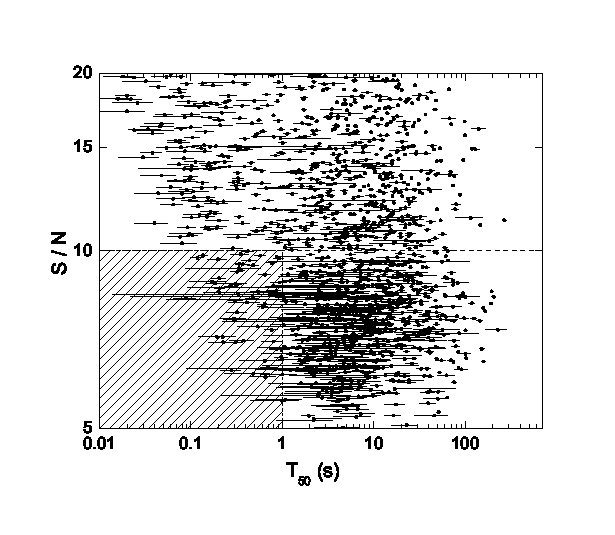
\includegraphics [width=0.8\textwidth] {gSNvsT50.eps}
  \caption[Соотношение S/N--$T_{50}$.]{Соотношение S/N--$T_{50}$ для 1834 всплесков. 
  Пунктирная линия соответствует $\rmn{S/N}=10$. Штрихованная область наиболее подвержена 
  селекции триггерного алгоритма. Отношение сигнал-шум $\rmn{S/N}\geq 10$ имеют 1168 всплесков.} 
  \label{img:SNvsT50}  
\end{figure}

\begin{figure}[h]
  \begin{minipage}[h]{0.5\textwidth}
    \center{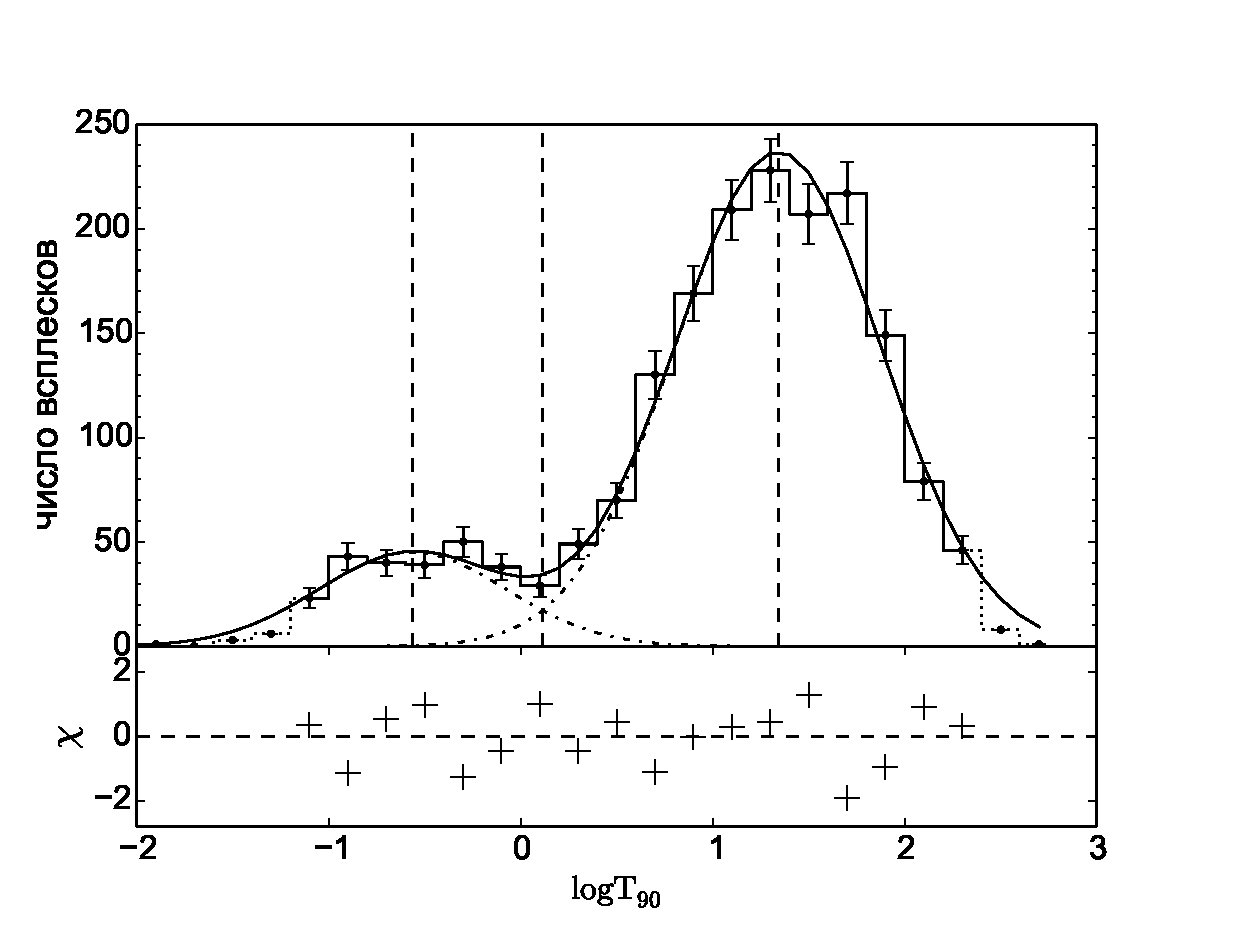
\includegraphics[width=1.0\textwidth]{dT90s5simple} \\ а)}
  \end{minipage}
  \hfill
  \begin{minipage}[h]{0.5\textwidth}
    \center{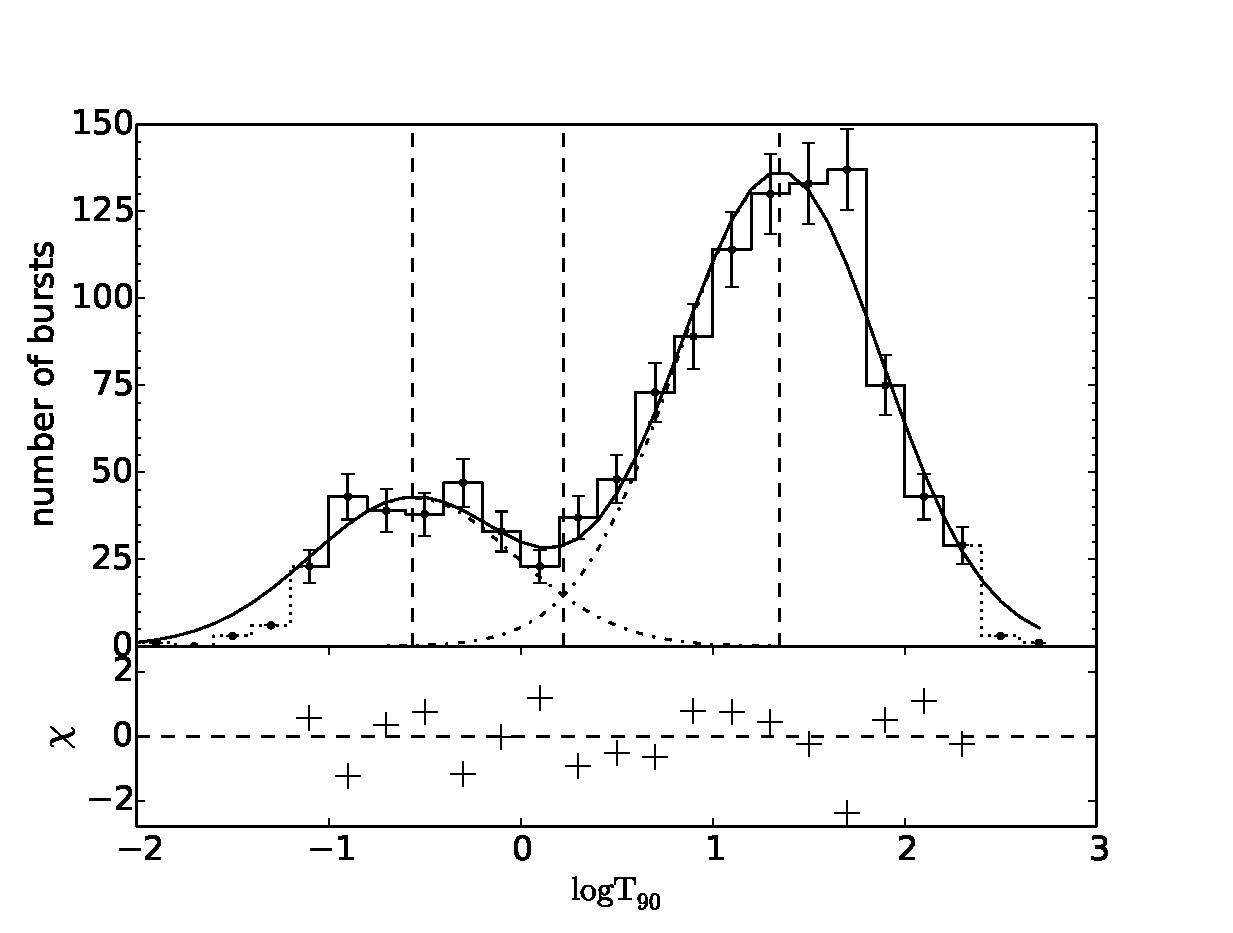
\includegraphics[width=1.0\textwidth]{dT90s5simple_SN10} \\ б)}
  \end{minipage}
  \vfill
  \begin{minipage}[h]{0.5\textwidth}
    \center{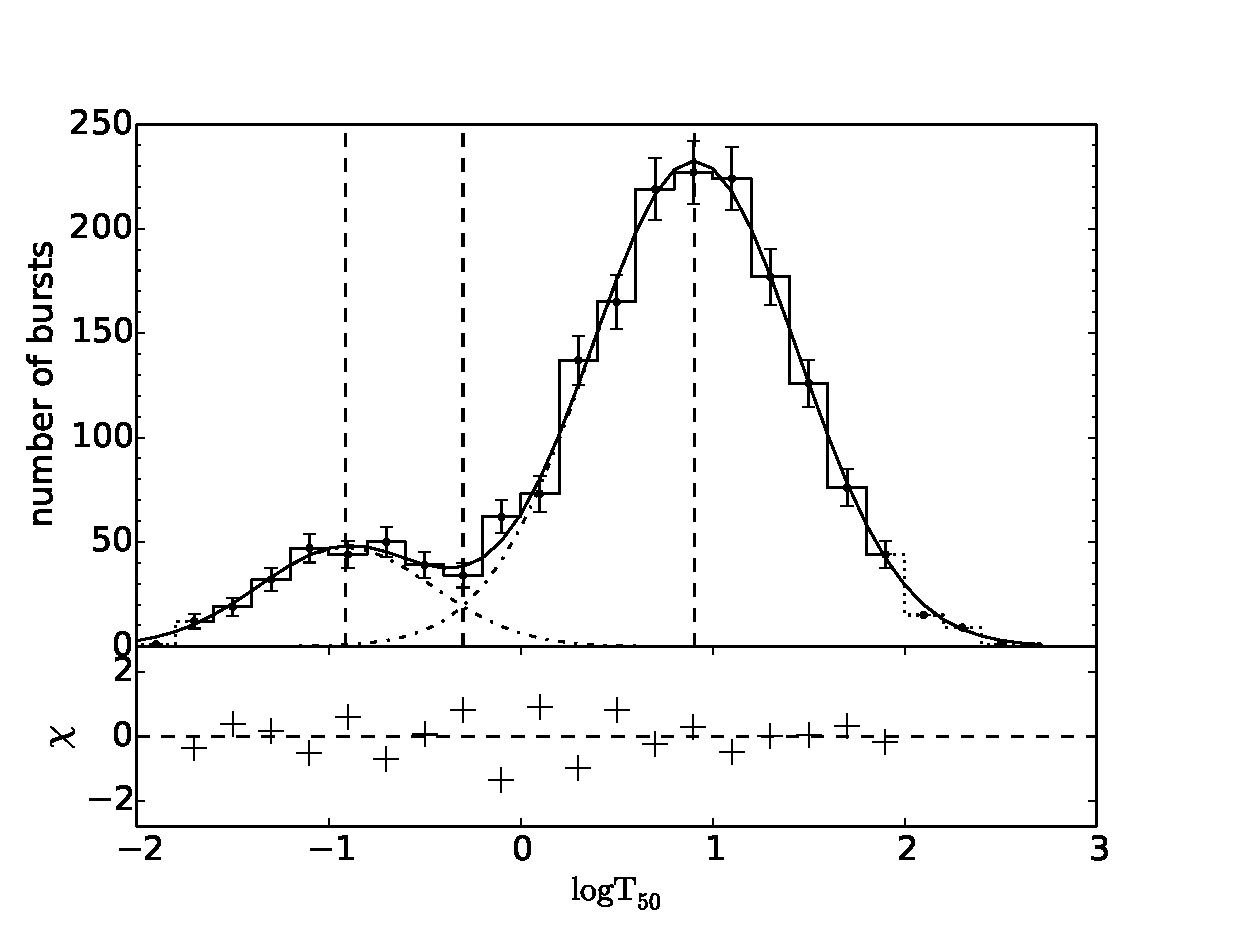
\includegraphics[width=1.0\textwidth]{dT50s5simple} \\ в)}
  \end{minipage}
  \hfill
  \begin{minipage}[h]{0.5\textwidth}
    \center{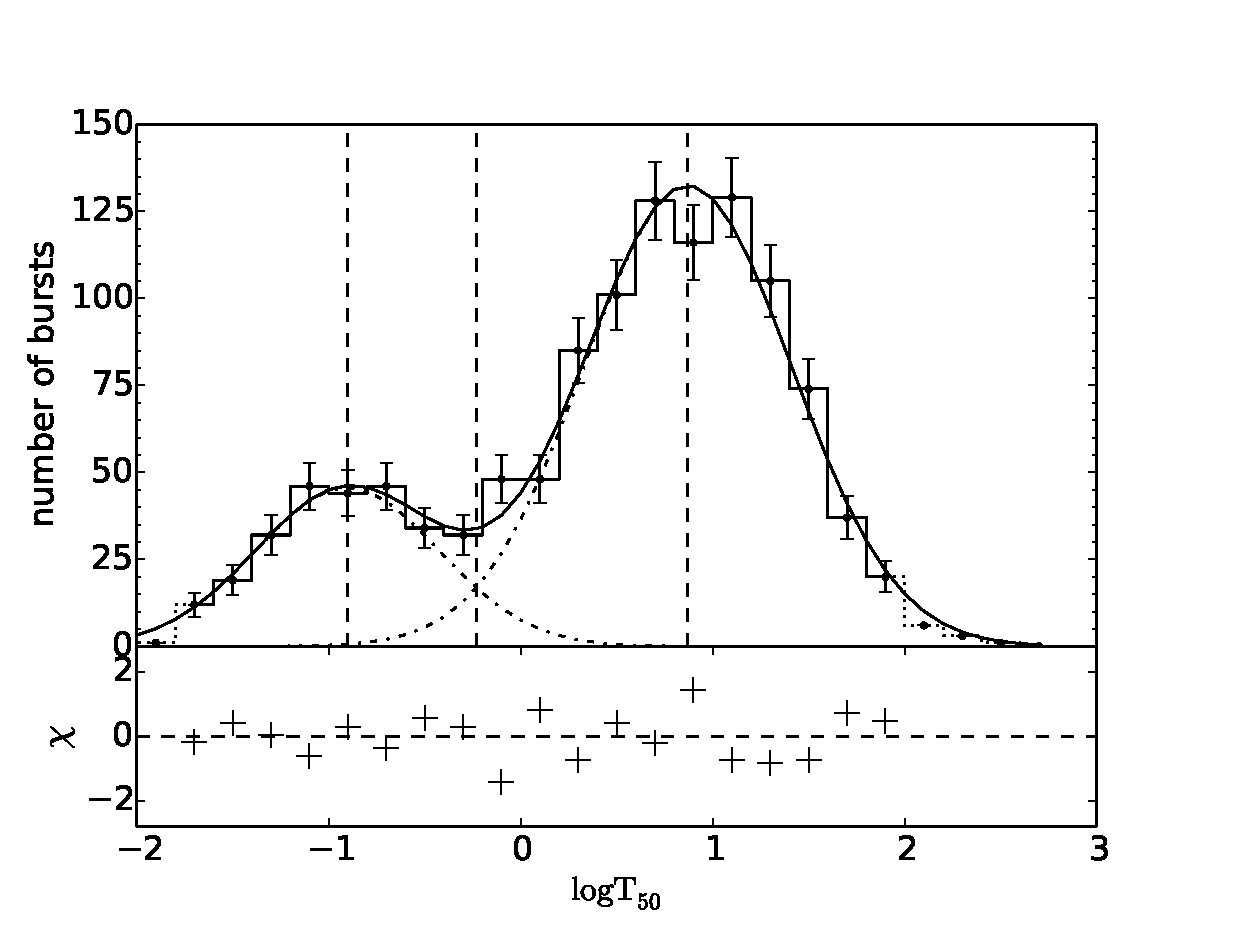
\includegraphics[width=1.0\textwidth]{dT50s5simple_SN10} \\ г)}
  \end{minipage}
  \caption[Распределения 1834-х и 1168-и всплесков с $\rmn{S/N}\geq 10$ по $T_{90}$ и~$T_{50}$]
  {Распределения 1834-х и 1168-и всплесков с $\rmn{S/N}\geq 10$ по $T_{90}$ (а, б) и 
  $T_{50}$ (в, г) для порога $5\sigma$ (непрерывная гистограмма), 
  игнорированные при аппроксимации бины гисторграммы показаны пунктиром. 
  Аппроксимация распределения суммой двух логнормальных распределений  показана 
  непрерывной линией, распределение коротких и длинных всплесков показаны 
  штрихпунктирными линиями.  Вертикальные штриховые лини обозначают средние значения 
  распределений коротких и длинных всплесков и точку их пересечения. 
  На нижней панели каждого рисунка показаны невязки аппроксимации.}
  \label{img:T90andT50s5}  
\end{figure}

\begin{landscape}
%\documentclass[preprint]{aastex}
%\usepackage{graphicx,natbib} 

%\begin{document}

\begin{table} [h]
 \centering
 \caption{Параметры аппроксимации распределений по $T_{90}$ для порогов 
          $4\sigma$, $5\sigma$ и $6\sigma$}\label{tab:T90_distr}
\scriptsize
%\rotate
  \begin{center}
  \begin{tabular}{c c c c c c c c c c c c c c} %14 col
  \hline
  \hline
число & $\sigma$ & $A_1$ & $xc_1$ & $T_{90c1}$ & $w_1$ & 
                 $A_2$ & $xc_2$ & $T_{90c2}$ & $w_2$ & 
				 $x_{\rmn{int}}$ & $T_{90\rmn{int}}$ & $\chi^2$ & dof \\
всплесков & & & & с & & & & с & & &  с & & \\
  \hline
%N_short = 243 N_long = 1591 N_tot = 1834
1834 & 4 & $     50 ^{+     6}_{-     5}$ & $  -0.49 ^{+  0.06}_{-  0.05}$ & $   0.32 ^{+  0.05}_{-  0.03}$ & $   0.92 ^{+  0.16}_{-  0.12}$ & $    324 ^{+     9}_{-    11}$ & $   1.44 ^{+  0.02}_{-  0.02}$ & $  27.30 ^{+  1.15}_{-  1.17}$ & $   1.11 ^{+  0.04}_{-  0.04}$ & $   0.15 ^{+  0.07}_{-  0.06}$ & $  1.42 ^{+ 0.26}_{- 0.19}$ &   10.5 & 12 \\ 
%N_short = 259 N_long = 1575 N_tot = 1834
& 5 & $     54 ^{+     8}_{-     6}$ & $  -0.56 ^{+  0.06}_{-  0.05}$ & $   0.27 ^{+  0.04}_{-  0.03}$ & $   0.97 ^{+  0.21}_{-  0.12}$ & $    316 ^{+     9}_{-    10}$ & $   1.34 ^{+  0.02}_{-  0.02}$ & $  22.09 ^{+  0.89}_{-  0.90}$ & $   1.06 ^{+  0.04}_{-  0.04}$ & $   0.11 ^{+  0.07}_{-  0.06}$ & $  1.30 ^{+ 0.24}_{- 0.16}$ &   14.6 & 12 \\ 
%N_short = 274 N_long = 1560 N_tot = 1834
& 6 & $     59 ^{+     8}_{-     6}$ & $  -0.59 ^{+  0.05}_{-  0.05}$ & $   0.26 ^{+  0.03}_{-  0.03}$ & $   0.95 ^{+  0.16}_{-  0.13}$ & $    312 ^{+     9}_{-    10}$ & $   1.30 ^{+  0.02}_{-  0.02}$ & $  20.00 ^{+  0.91}_{-  0.74}$ & $   1.07 ^{+  0.04}_{-  0.04}$ & $   0.09 ^{+  0.07}_{-  0.06}$ & $  1.22 ^{+ 0.22}_{- 0.15}$ &   10.3 & 12 \\ 
%N_short = 248 N_long = 920 N_tot = 1168
1168& 4 & $     53 ^{+    11}_{-     7}$ & $  -0.47 ^{+  0.10}_{-  0.06}$ & $   0.34 ^{+  0.09}_{-  0.05}$ & $   1.03 ^{+  0.31}_{-  0.18}$ & $    182 ^{+    10}_{-    12}$ & $   1.42 ^{+  0.03}_{-  0.03}$ & $  26.41 ^{+  2.12}_{-  1.85}$ & $   1.07 ^{+  0.07}_{-  0.08}$ & $   0.28 ^{+  0.15}_{-  0.12}$ & $  1.91 ^{+ 0.81}_{- 0.45}$ &   13.2 & 12 \\ 
%N_short = 264 N_long = 904 N_tot = 1168
S/N$>$10 & 5 & $     58 ^{+    10}_{-     8}$ & $  -0.57 ^{+  0.08}_{-  0.07}$ & $   0.27 ^{+  0.05}_{-  0.04}$ & $   1.09 ^{+  0.29}_{-  0.20}$ & $    178 ^{+     9}_{-    10}$ & $   1.35 ^{+  0.03}_{-  0.03}$ & $  22.51 ^{+  1.74}_{-  1.41}$ & $   1.05 ^{+  0.06}_{-  0.06}$ & $   0.23 ^{+  0.13}_{-  0.10}$ & $  1.71 ^{+ 0.58}_{- 0.36}$ &   15.5 & 12 \\ 
%N_short = 278 N_long = 890 N_tot = 1168
& 6 & $     61 ^{+    12}_{-     7}$ & $  -0.60 ^{+  0.06}_{-  0.06}$ & $   0.25 ^{+  0.04}_{-  0.04}$ & $   1.04 ^{+  0.29}_{-  0.16}$ & $    175 ^{+     7}_{-    10}$ & $   1.32 ^{+  0.03}_{-  0.03}$ & $  20.79 ^{+  1.54}_{-  1.28}$ & $   1.04 ^{+  0.06}_{-  0.06}$ & $   0.21 ^{+  0.11}_{-  0.10}$ & $  1.63 ^{+ 0.49}_{- 0.32}$ &   16.1 & 12 \\ 
\hline
\end{tabular}
\end{center}
\end{table}

\begin{table} [h]
 \centering
 \caption{Параметры аппроксимации распределений по $T_{50}$ для порогов 
          $4\sigma$, $5\sigma$ и $6\sigma$}\label{tab:T50_distr}
\scriptsize
%\rotate
  \begin{center}
  \begin{tabular}{c c c c c c c c c c c c c c}
  \hline
  \hline
число всплесков & $\sigma$ & $A_1$ & $xc_1$ & $T_{90c1}$ & $w_1$ & 
                             $A_2$ & $xc_2$ & $T_{90c2}$ & $w_2$ & 
							 $x_{\rmn{int}}$ & $T_{90\rmn{int}}$ & $\chi^2$ & dof \\
							 
всплесков & & & & с & & & & с & & &  с & & \\
\hline
%N_short = 252 N_long = 1582 N_tot = 1834
1834 & 4 & $     50 ^{+     5}_{-     4}$ & $  -0.86 ^{+  0.05}_{-  0.05}$ & $   0.14 ^{+  0.02}_{-  0.01}$ & $   0.86 ^{+  0.10}_{-  0.09}$ & $    312 ^{+     9}_{-     9}$ & $   0.95 ^{+  0.02}_{-  0.02}$ & $   8.86 ^{+  0.36}_{-  0.35}$ & $   1.06 ^{+  0.04}_{-  0.04}$ & $  -0.26 ^{+  0.06}_{-  0.06}$ & $  0.54 ^{+ 0.08}_{- 0.07}$ &   14.7 & 13 \\ 
%N_short = 263 N_long = 1571 N_tot = 1834
& 5 & $     53 ^{+     6}_{-     5}$ & $  -0.91 ^{+  0.05}_{-  0.05}$ & $   0.12 ^{+  0.02}_{-  0.01}$ & $   0.89 ^{+  0.12}_{-  0.10}$ & $    311 ^{+    10}_{-     9}$ & $   0.91 ^{+  0.02}_{-  0.02}$ & $   8.06 ^{+  0.35}_{-  0.33}$ & $   1.07 ^{+  0.04}_{-  0.04}$ & $  -0.30 ^{+  0.07}_{-  0.06}$ & $  0.50 ^{+ 0.09}_{- 0.07}$ &    6.9 & 13 \\ 
%N_short = 278 N_long = 1556 N_tot = 1834
& 6 & $     57 ^{+     6}_{-     5}$ & $  -0.89 ^{+  0.06}_{-  0.05}$ & $   0.13 ^{+  0.02}_{-  0.02}$ & $   0.93 ^{+  0.12}_{-  0.10}$ & $    307 ^{+    10}_{-     9}$ & $   0.89 ^{+  0.02}_{-  0.02}$ & $   7.73 ^{+  0.35}_{-  0.34}$ & $   1.07 ^{+  0.04}_{-  0.04}$ & $  -0.28 ^{+  0.07}_{-  0.07}$ & $  0.52 ^{+ 0.09}_{- 0.08}$ &    8.4 & 13 \\ 
%N_short = 256 N_long = 912 N_tot = 1168
1168 &4 & $     51 ^{+     6}_{-     5}$ & $  -0.85 ^{+  0.07}_{-  0.06}$ & $   0.14 ^{+  0.02}_{-  0.02}$ & $   0.92 ^{+  0.13}_{-  0.12}$ & $    178 ^{+     8}_{-     9}$ & $   0.91 ^{+  0.03}_{-  0.03}$ & $   8.07 ^{+  0.55}_{-  0.51}$ & $   1.05 ^{+  0.06}_{-  0.05}$ & $  -0.19 ^{+  0.09}_{-  0.09}$ & $  0.65 ^{+ 0.15}_{- 0.12}$ &   15.8 & 13 \\ 
%N_short = 263 N_long = 905 N_tot = 1168
S/N$>$10 &  5 & $     54 ^{+     7}_{-     6}$ & $  -0.90 ^{+  0.08}_{-  0.06}$ & $   0.12 ^{+  0.03}_{-  0.01}$ & $   0.94 ^{+  0.17}_{-  0.12}$ & $    178 ^{+     7}_{-     9}$ & $   0.87 ^{+  0.03}_{-  0.03}$ & $   7.43 ^{+  0.58}_{-  0.51}$ & $   1.07 ^{+  0.06}_{-  0.06}$ & $  -0.23 ^{+  0.11}_{-  0.09}$ & $  0.59 ^{+ 0.17}_{- 0.11}$ &    9.3 & 13 \\ 
%N_short = 278 N_long = 890 N_tot = 1168
& 6 & $     56 ^{+     7}_{-     6}$ & $  -0.89 ^{+  0.07}_{-  0.06}$ & $   0.13 ^{+  0.02}_{-  0.02}$ & $   0.96 ^{+  0.14}_{-  0.11}$ & $    175 ^{+     7}_{-     8}$ & $   0.86 ^{+  0.03}_{-  0.03}$ & $   7.29 ^{+  0.52}_{-  0.48}$ & $   1.06 ^{+  0.06}_{-  0.05}$ & $  -0.21 ^{+  0.09}_{-  0.08}$ & $  0.61 ^{+ 0.15}_{- 0.11}$ &    9.6 & 13 \\ 
\hline
\end{tabular}
\end{center}
\end{table}
%\end{document}

\end{landscape}

\subsection{Сравнение длительностей определенных по данным BATSE и Конус-Винд}
Среди 1939 всплесков Конус-Винд без сбоев 267 всплесков наблюдались BATSE. 
Соотношение длительностей $T_{50}$ и $T_{90}$, вычисленных по данным BATSE~\citep{Paciesas_1999} 
и Конус-Винд, изображено на рис.~\ref{img:T90andT50_KWvsBATSE}.

Большинство всплесков имеют б\'{о}льшую длительность по данным BATSE, 
в особенности $T_{90}$, что связано с большей  эффективной площадью детекторов 
BATSE $\sim 10^3$~см$^2$ против 0.80--$1.6\times 10^2$~см$^2$ у Конус-Винд. 
Другим фактором является то, что длительность всплесков BATSE определяется в 
диапазоне $>25$~кэВ, что позволяет учитывать продолжительные мягкие хвосты всплесков. 
Более редкой ситуацией является существенное превышение длительностей по данным Конус-Винд, 
наблюдаемое в 10 всплесках. Шесть всплесков имеют плавное спадание/нарастание интенсивности, 
которое не было учтено при вычислении  длительностей по данным BATSE, возможно, 
из-за недостаточно точной аппроксимации фона. В трех всплесках по данным Конус-Винд 
в интервал $T_{90}$ попадает слабый импульс, отделенный от основного пика. 
При этом эклиптические широты основного пика и слабого импульса согласуются, 
что позволяет отнести их к одному источнику. Во всплеске GRB~950904, 
$T_{0 \rmn{BATSE}} = 52777$~s~UT ($T_{90{KW}} = 99 \pm 4$~с, $T_{90\rmn{BATSE}} = 11.1\pm 1.8$~с) 
длительности BATSE даны для второго импульса, так как в~\citep{Hurley_2005} полагается, 
что два импульса являются различными всплесками.

Среди общих всплесков Конус-Винд и BATSE 46 имеют $T_{50{KW}} \leq 0.6$~с. 
В наш список коротких всплесков входят 37 из них, оставшиеся 9 входят в список из 105 
всплесков с искаженной длительностью. Из 37 коротких всплесков у восьми $T_{90\rmn{BATSE}} > 2$~с, 
из них один является короткими всплеском с продлённым излучением. Таким образом, 
засорение нашего списка длинными всплесками составляет 19\% (7/37), без учета 
всплесков с продлённым излучением. Ранее в~\citep{Ofek_2007} была получена доля 
<<засорения>> коротких всплесков Конус-Винд длинными $\sim 60$\%. В этой работе 
длительность всплесков в данных Конус-Винд оценивалась визуально, что могло 
стать причиной завышения доли засорения. 

\begin{figure}[h]
  \begin{minipage}[h]{0.5\textwidth}
    \center{\includegraphics[width=1.0\textwidth]{gT90_KWvsBATSE} \\ а)}
  \end{minipage}
  \hfill
  \begin{minipage}[h]{0.5\textwidth}
    \center{\includegraphics[width=1.0\textwidth]{gT50_KWvsBATSE} \\ б)}
  \end{minipage}
  \caption{Соотношение длительностей $T_{90}$ (a) и $T_{50}$ (б), определённых по 
  данным BATSE и Конус-Винд для 267 гамма-всплесков.}
  \label{img:T90andT50_KWvsBATSE}  
\end{figure}

\subsection{Набор коротких всплесков}
Наш набор из 1834 всплесков содержит 273 событий с $T_{50} \leq 0.6$~c. 
Среди них было обнаружено четыре очевидно длинных всплеска: два с сильным коротким 
импульсом в середине всплеска~\textbf{(ID=2196, 2922)}, один всплеск с сильным мягким 
предшественником и слабым импульсом на $\sim T_0+100$~с~\textbf{(ID=1122)}, 
и один всплеск с интенсивным начальным импульсом и слабым вторым импульсом на 
$\sim T_0+5$~с~\textbf{(ID=2184)}. Также был исключён всплеск~\textbf{(ID=1228)}, 
у которого по данным \textit{BeppoSAX} $T_{90} = 8$~с. Визуальный анализ показал, 
что среди 69 всплесков со сбоями три имеют $T_{50} \leq 0.6$~c. Таким образом, 
набор коротких всплесков Конус-Винд содержит 273 всплеска.

Кроме того, было обнаружено 23 всплеска с продлённым излучением. К этому типу 
всплесков мы отнесли события, имеющие короткий начальный импульс $T_{50} \leq 0.6$, 
за которым следует более мягкий и менее интенсивный эпизод 
излучения~\citep{Frederiks_2004ASPC, Norris_2011ApJ, Norris_and_Bonnel_2006}. 
В некоторых случаях начальный пик и продлённое излучение разделены интервалом, 
на котором интенсивность излучения мала.

Объединённый набор коротких всплесков с учётом всплесков с продлённым излучением 
содержит 296 всплесков.

\clearpage

\section{Жесткости}\label{sec:Hardness}
Для анализа спектральных различий всплесков мы использовали две величины: интегральную 
жесткость ($\rmn{HR}_{32}$)~--- отношение числа отсчетов, накопленных в каналах G3 и G2 
за интервал $T_{100}$ и пиковую жесткость ($\rmn{HR}_{32\rmn{pk}}$)~--- отношение числа отсчетов, 
накопленных за интервал 64~мс с пиковой скоростью счета. Для нашего набора 
всплесков мы использовали отношение числа отсчётов в каналах G3 и G2 так как 
оно наименее чувствительно к углу падения на детектор и более чувствительно 
к пиковой энергии $E_{\rmn{p}}$.  

При вычислении жесткости $\rmn{HR}_{32}$ был учтён временн\'{о}й дрейф границ диапазонов. 
Для этого трёхканальный спектр отсчётов аппроксимировался степенной функцией 
с экспоненциальным завалом $dN/dE \propto E^{-\alpha} \exp(-E/E_0)$. 
С использованием полученной аппроксимации, вычислялось количество отсчётов в номинальных 
границах диапазонов: 12--50~кэВ~(G1), 50--200~кэВ~(G2) и 200--750~кэВ~(G3). 
Реальные границы диапазонов были вычислены с использованием калибровки, полученной 
по многоканальному спектру.  Многоканальный спектр калибровался по линии 
радиоактивного изотпа $^{40}$K, содержащегося в веществе детектора.

При рассмотрении интегральной жесткости использовался однородный набор из 1168 
всплесков с $\rmn{S/N} \geq 10$. Набор содержит восемь всплесков со сбоями в G1, 
для которых невозможно провести аппроксимацию трёхканального спектра. 
Из оставшихся всплесков, 17 имеют значительную неопределённость HR$_{32}$ 
($\sigma\rmn{HR}_{32}/\rmn{HR}_{32} >0.3$), и они были исключены из рассмотрения. 
В итоге для исследования соотношения жесткость-длительность использовалось 1143 всплеска.

Аналогично~\citep{Horvath_2006} мы аппроксимировали распределения всплесков на 
плоскости $\log T_{50}$--$\log \rmn{HR}_{32}$ используя сумму двух и трёх 
гауссовых компонент. В отличие от предыдущих работ мы использовали меру длительности 
$T_{50}$, так как выше было показано, что эта мера длительности более предпочтительна 
для классификации, чем $T_{90}$. Каждая компонента имеет вид: 
\begin{equation}
p(x,y| l) = \frac{1}{2\pi \sigma_x \sigma_y \sqrt{1-r^2}} \times 
\exp\left[ -\frac{1}{2(1-r^2)}\left( \frac{(x-a_x)^2}{\sigma_x^2} + 
\frac{(y-a_y)^2}{\sigma_y^2} -\frac{C}{\sigma_x \sigma_y}\right)\right]\mbox{ ,}
\end{equation}
где
\begin{equation}
C = 2r(x-a_x)(y-a_y)\mbox{ ,} \nonumber
\end{equation}
где $x=\log T_{50}$ и $y=\log \mbox{HR}_{32}$,  $a_x$, $a_y$~--- средние, 
$\sigma_x$, $\sigma_y$~--- дисперсии, $r$~--- коэффициент корреляции, 
и $l$~--- номер компоненты. При этом функция правдоподобия определяется следующим образом:
\begin{equation}
L = \sum_i \ln p(x_i, y_i)\mbox{ ,}
\end{equation}
где
\begin{equation}
p(x,y) = \sum_l  p(x, y|l)p_l \nonumber
\end{equation}
Аппроксимация производилась с помощью алгоритма 
expectation-maximization~\citep{Horvath_2006, Balazs_2003AA} реализованного в пакете 
Scikit-learn~\citep{scikit-learn}.  Принадлежность всплеска к классу $l$ определяется 
на основании наибольшего значения индикаторной функции
\begin{equation}
I_l =\frac{p_l p(x,y|l)}{\sum_l  p(x, y|l)}
\end{equation}
Ошибки параметров вычислялись таким же методом, как и для распределения по длительностям. 
На каждой и 1000 итераций генерировалось распределение на плоскости  
$\log T_{50}$--$\log\rmn{HR}_{32}$ на основе ошибок $T_{50}$ и $\rmn{HR}_{32}$. 
Затем из полученных распределений параметров в качестве значения и ширины доверительного 
интервала бралась медиана и ширина на уровне 68\%. Значения параметров распределений 
для случая двух и трёх компонент представлены в таблицах~\ref{tab:clusters2_HR} 
и~\ref{tab:clusters3_HR}, расположение компонент представлено на рис.~\ref{img:HRvsT50}. 

Различие значений функций правдоподобия для двух компонент $L_2 = -1243$ и трёх 
компонент $L_3 = -1219$ ($\Delta L = 24$). Как показано в~\citep{Horvath_2006} 
в этом случае $2\Delta L$ распределено как $\chi^2_6$ и вероятность случайного 
отклонения $2\Delta L = 48$ равна $10^{-8}$. Функция правдоподобия для четырёх 
компонент $L_4 = -1211$, $2(L_4 - L_3) = 16$ этой величине соответствует вероятность $0.01$. 
Это свидетельствует о наличии не более трёх классов всплесков. Третий класс всплесков 
значительно перекрывается с классом длинных/мягких всплесков, поэтому нельзя утверждать, 
что он соответствует реальному физически выделенному классу всплесков. На основании 
этого для дальнейшего описание набора всплесков Конус-Винд используется только 
два класса всплесков: короткие/жесткие и длинные/мягкие.

Полученный класс коротких/жестких всплесков содержит 232 всплеска. Из этих 
всплесков 6 имеют $T_{50} > 0.6$~с. Для временной истории этих всплесков характерно 
наличие нескольких импульсов с резким нарастанием и спадом.  Класс длинных всплесков 
содержит 911 всплесков, из которых 34 достаточно мягких с длительностью 0.1~c~$< T_{50} <=0.6$~с. 
Эти 34 всплеска в основном содержат один пологий импульс. Полученная доля коротких 
всплесков составляет 21\% (таб.~\ref{tab:clusters2_HR}). Доля всплесков, отнесенных 
к классу длинных/мягких всплесков, среди всплесков с $T_{50} \leq 0.6$~с  равна 13\% (34/260). 
Из 23-х коротких всплесков с продлённым излучением начальные импульсы двух 
событий \textbf{(ID = 544, 1531)} принадлежат к классу длинных/мягких всплесков.

Такой же анализ был проведен и для распределения длительность-пиковая жесткость. 
Для этого использовались 1104 GRBs с $\rmn{S/N} \geq 10$ и $\sigma \rmn{HR}_{32\rmn{pk}}/\rmn{HR}_{32\rmn{pk}} <0.3$. 
Результат аппроксимации двумя гауссовыми компонентами приведен на рис.~\ref{img:HRpkvsT50}. 
Параметры распределений приведены в таблице~\ref{tab:tab_2clusters_HRpk} и~\ref{tab:tab_3clusters_HRpk}. 

Различие в жесткостях длинных и коротких составляет 1.7 раза для пиковых 
жесткостей и 2.4 раза для интегральных. 

%\documentclass[preprint]{aastex}
%\usepackage{graphicx,natbib} 
%
%\begin{document}

\begin{table} [h]
 \centering
 \caption{Параметры распределения $\log T_{50}$--$\log \rmn{HR}_{32}$, в случае $k=2$}\label{tab:clust_2}
\scriptsize

  \begin{center}
  \begin{tabular}{c c c c c c c c c}
  \hline
  \hline
$l$  &  $a_x$ &  $T_{50c}$ (c) &  $a_y$ &   $\rmn{HR}_c$ &  $\sigma_x$ &  $\sigma_y$ &  $r$ &  $p_l$\\
  \hline
1 & $-0.940_{-  0.012}^{+  0.032}$ & $   0.115_{-  0.003}^{+  0.009}$ & $-0.124_{-  0.019}^{+  0.011}$ & $   0.752_{-  0.032}^{+  0.020}$ & $ 0.442_{-  0.015}^{+  0.033}$ & $ 0.221_{-  0.010}^{+  0.008}$ & $ 0.020_{-  0.056}^{+  0.041}$ & $ 0.210_{-  0.003}^{+  0.011}$\\
2 & $ 0.835_{-  0.005}^{+  0.017}$ & $   6.834_{-  0.081}^{+  0.265}$ & $-0.499_{-  0.002}^{+  0.001}$ & $   0.317_{-  0.002}^{+  0.001}$ & $ 0.560_{-  0.019}^{+  0.003}$ & $ 0.216_{-  0.003}^{+  0.003}$ & $ 0.176_{-  0.008}^{+  0.006}$ & $ 0.791_{-  0.012}^{+  0.002}$\\
  \hline
\end{tabular}
\end{center}
\end{table}

\begin{table} [h]
 \centering
 \caption{Параметры распределения $\log T_{50}$--$\log \rmn{HR}_{32}$, в случае $k=3$}\label{tab:clust_3}
\scriptsize

  \begin{center}
  \begin{tabular}{c c c c c c c c c}
  \hline
  \hline
$l$  &  $a_x$ &  $T_{50c}$ (c) &  $a_y$ &   $\rmn{HR}_c$ &  $\sigma_x$ &  $\sigma_y$ &  $r$ &  $p_l$\\
  \hline
1 & $-0.962_{-  0.016}^{+  0.008}$ & $   0.109_{-  0.004}^{+  0.002}$ & $-0.058_{-  0.013}^{+  0.003}$ & $   0.876_{-  0.026}^{+  0.005}$ & $ 0.414_{-  0.018}^{+  0.019}$ & $ 0.168_{-  0.016}^{+  0.007}$ & $ 0.098_{-  0.056}^{+  0.020}$ & $ 0.170_{-  0.010}^{+  0.009}$\\
2 & $ 0.088_{-  0.115}^{+  0.129}$ & $   1.224_{-  0.284}^{+  0.424}$ & $-0.583_{-  0.023}^{+  0.019}$ & $   0.261_{-  0.013}^{+  0.012}$ & $ 0.739_{-  0.030}^{+  0.031}$ & $ 0.264_{-  0.004}^{+  0.023}$ & $-0.176_{-  0.112}^{+  0.063}$ & $ 0.187_{-  0.017}^{+  0.006}$\\
3 & $ 0.949_{-  0.012}^{+  0.004}$ & $   8.886_{-  0.237}^{+  0.083}$ & $-0.468_{-  0.004}^{+  0.005}$ & $   0.340_{-  0.003}^{+  0.004}$ & $ 0.487_{-  0.003}^{+  0.005}$ & $ 0.194_{-  0.003}^{+  0.001}$ & $ 0.071_{-  0.004}^{+  0.009}$ & $ 0.654_{-  0.022}^{+  0.010}$\\
\hline
\end{tabular}
\end{center}
\end{table}

\begin{table} [h]
 \centering
 \caption{Параметры распределения $\log T_{50}$--$\log \rmn{HR}_{32\rmn{pk}}$, в случае $k=2$}\label{tab:pk_clust_2}
\scriptsize

  \begin{center}
  \begin{tabular}{c c c c c c c c c}
  \hline
  \hline
  $l$  &  $a_x$ &  $T_{50c}$ (c) &  $a_y$ &   $\rmn{HR}_c$ &  $\sigma_x$ &  $\sigma_y$ &  $r$ &  $p_l$\\
  \hline
1 & $-0.948_{-  0.012}^{+  0.025}$ & $   0.113_{-  0.003}^{+  0.007}$ & $-0.068_{-  0.008}^{+  0.008}$ & $   0.856_{-  0.016}^{+  0.016}$ & $ 0.422_{-  0.015}^{+  0.009}$ & $ 0.260_{-  0.008}^{+  0.002}$ & $ 0.112_{-  0.045}^{+  0.020}$ & $ 0.214_{-  0.003}^{+  0.003}$\\
2 & $ 0.842_{-  0.006}^{+  0.004}$ & $   6.954_{-  0.097}^{+  0.059}$ & $-0.286_{-  0.001}^{+  0.006}$ & $   0.517_{-  0.001}^{+  0.007}$ & $ 0.550_{-  0.004}^{+  0.001}$ & $ 0.248_{-  0.001}^{+  0.007}$ & $ 0.191_{-  0.013}^{+  0.002}$ & $ 0.786_{-  0.003}^{+  0.003}$\\
\hline
\end{tabular}
\end{center}
\end{table}
%\end{document}

\begin{figure}[h]
  \begin{minipage}[h]{0.5\textwidth}
    \center{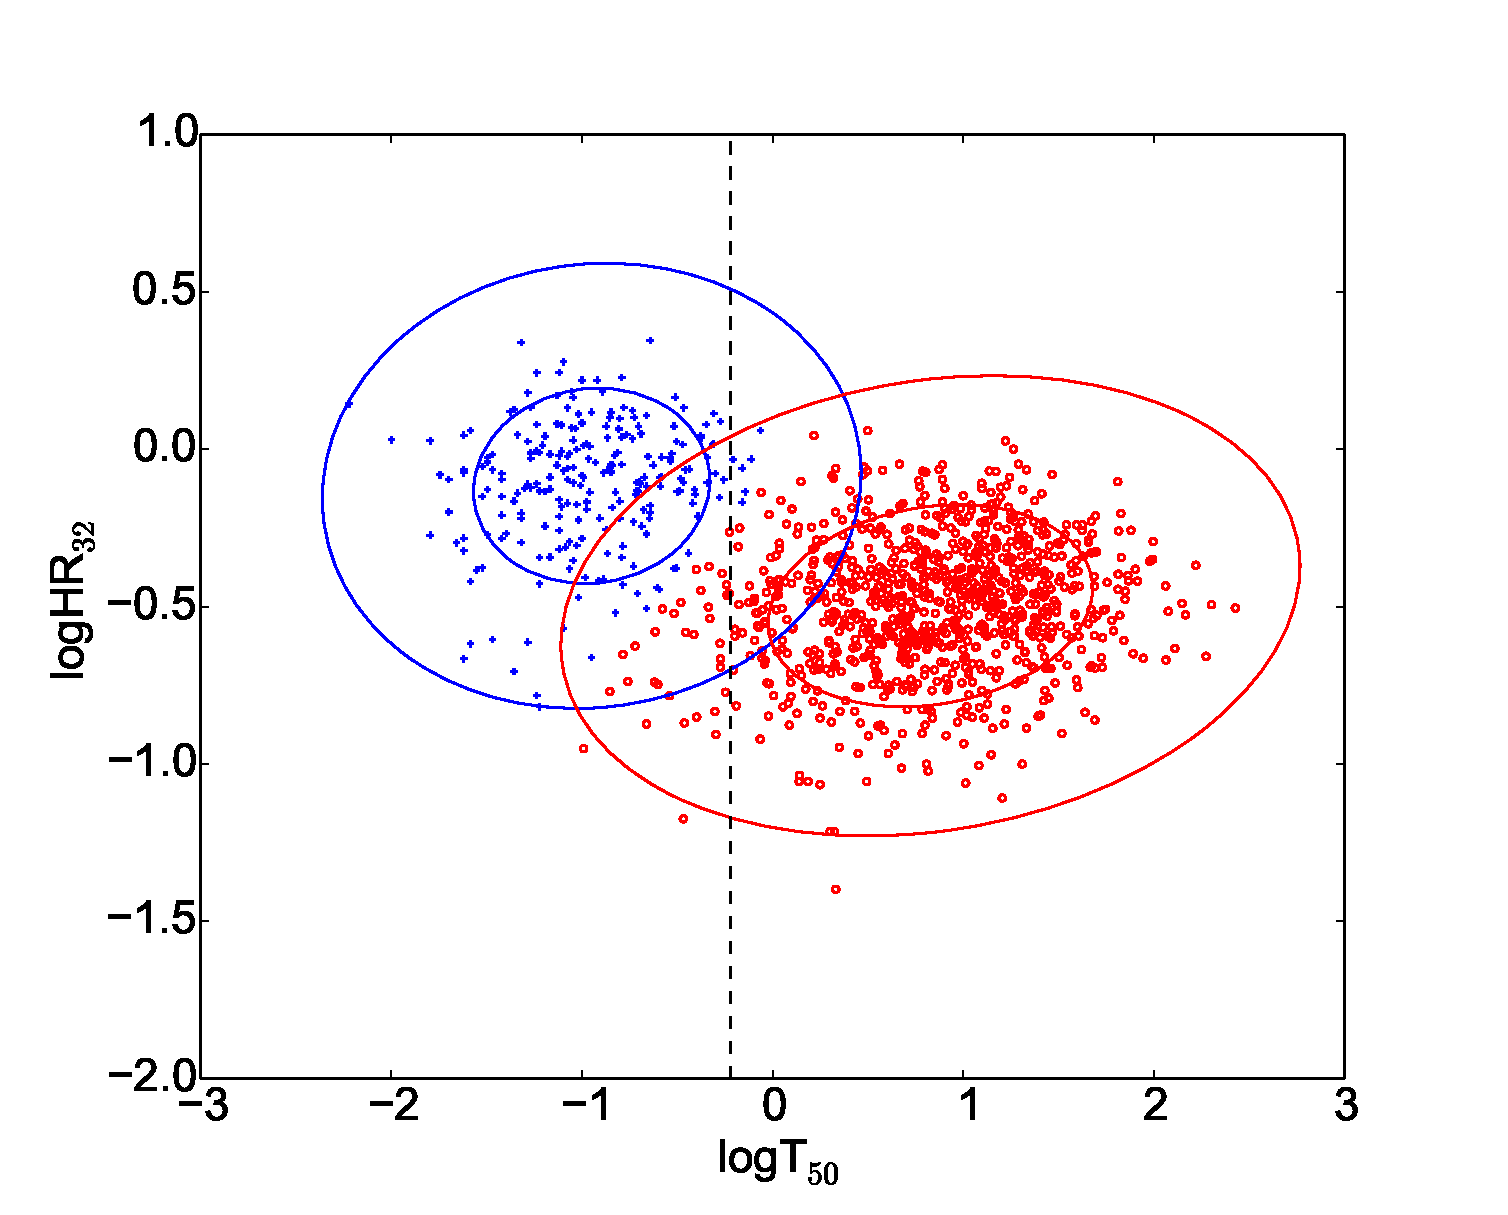
\includegraphics[width=1.0\textwidth]{list1143calHR_2} \\ а)}
  \end{minipage}
  \hfill
  \begin{minipage}[h]{0.5\textwidth}
    \center{\includegraphics[width=1.0\textwidth]{list1143calHR_3} \\ б)}
  \end{minipage}
  \caption[Аппроксимация распределения $\log T_{50}$--$\log \mbox{HR}_{32}$.]
  {Аппроксимация распределения $\log T_{50}$--$\log \mbox{HR}_{32}$ 
  для 1143 ярких ($\rmn{S/N} \geq 10$) всплесков двумя~(a) и тремя~(б) гауссовыми компонентами. 
  Эллипсами для каждого распределения отмечены области 1$\sigma$ и~3$\sigma$ сигма. 
  Пунктирная вертикальная линия~--- $T_{50} = 0.6$~с. Кресты~--- короткие/жесткие всплески, 
  круги~--- длинные/мягкие всплески, треугольники~--- промежуточные всплески.}
  \label{img:HRvsT50}  
\end{figure}

\begin{figure}[h]
  \begin{minipage}[h]{0.5\textwidth}
    \center{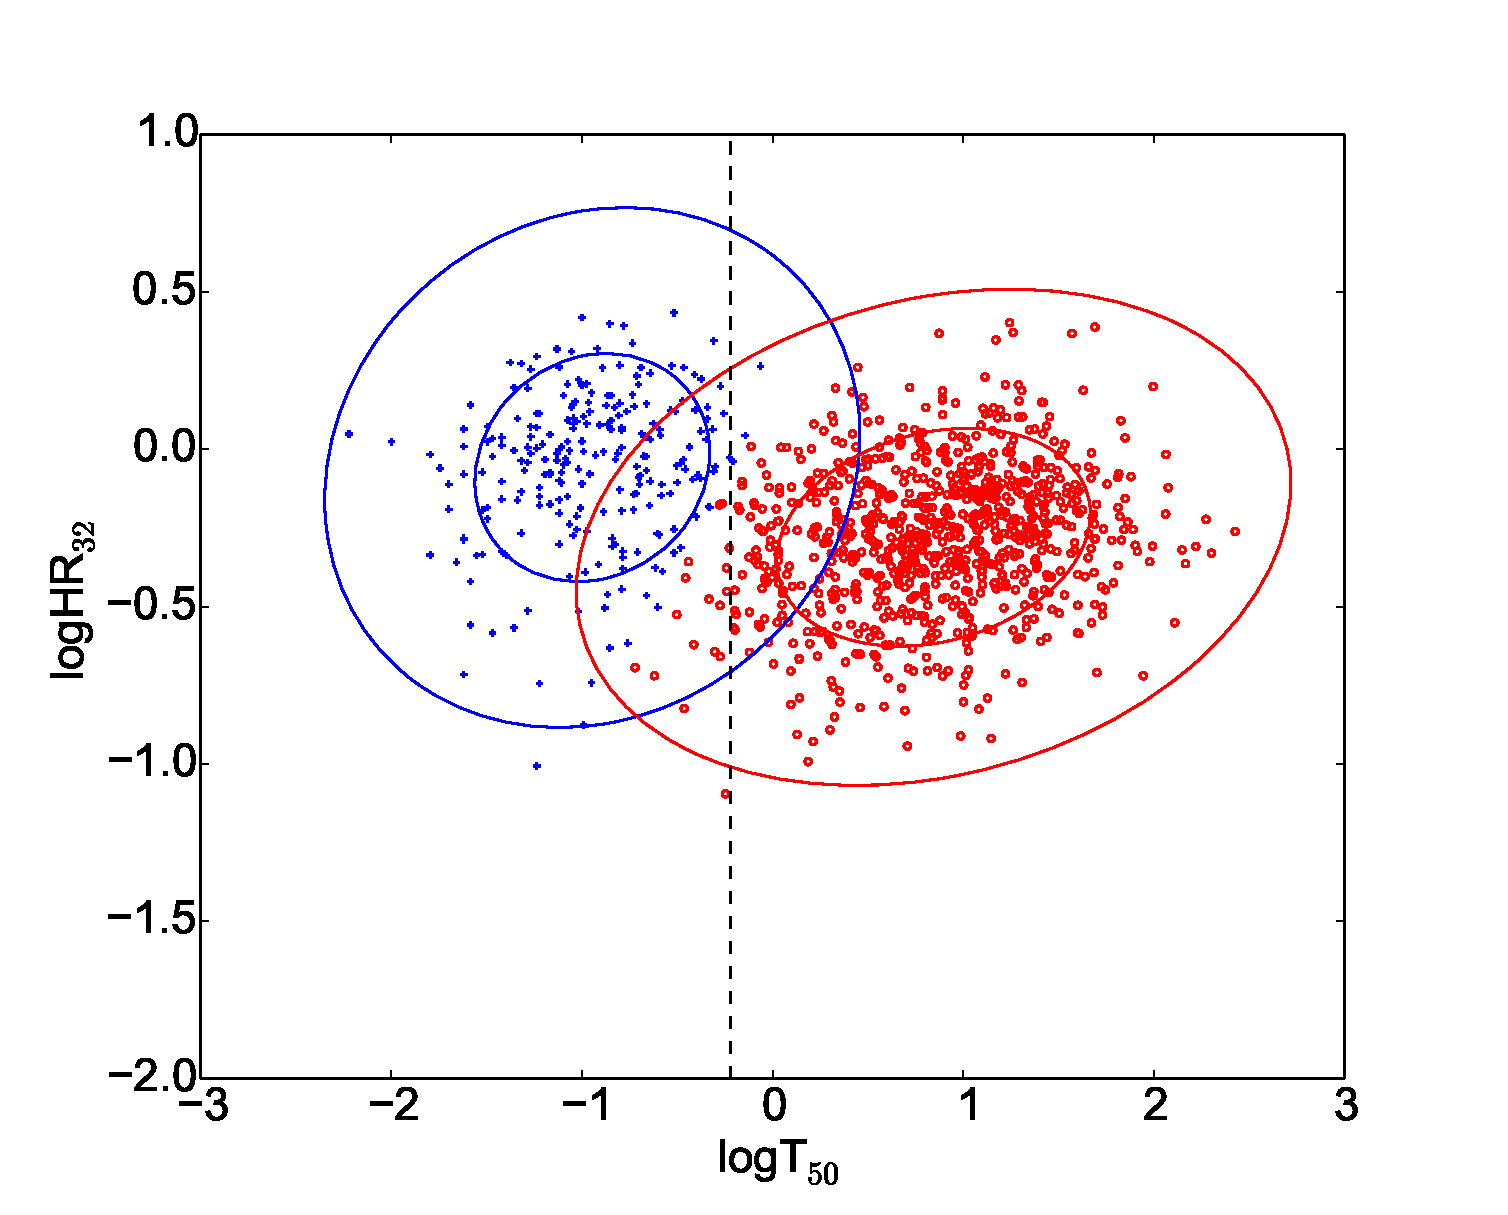
\includegraphics[width=1.0\textwidth]{list1104calHRpcr_2} \\ а)}
  \end{minipage}
  \hfill
  \begin{minipage}[h]{0.5\textwidth}
    \center{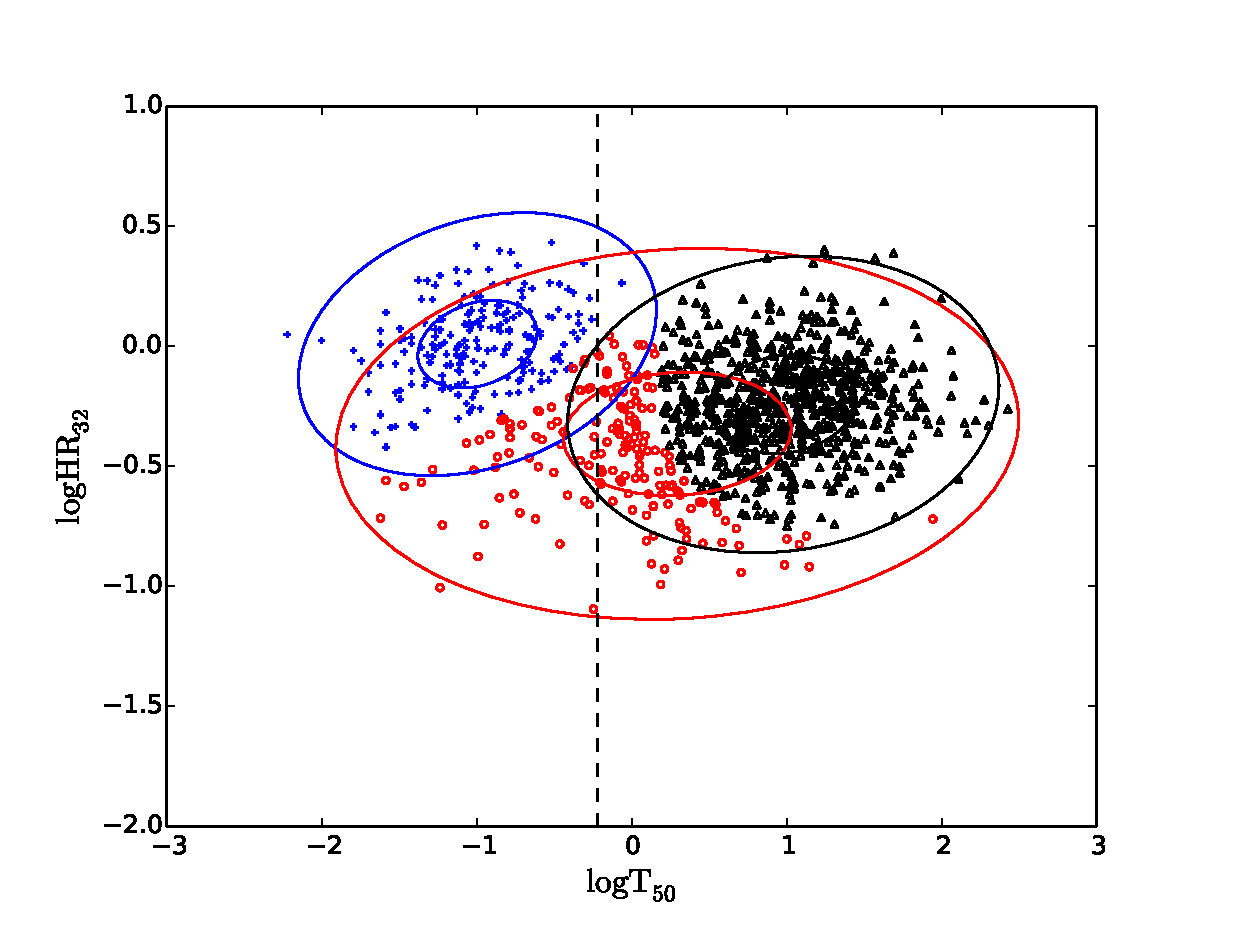
\includegraphics[width=1.0\textwidth]{list1104calHRpcr_3} \\ б)}
  \end{minipage}
  \caption[Аппроксимация распределения $\log T_{50}\textrm{--}\log \mbox{HR}_{32\rmn{pk}}$.]
  {Аппроксимация распределения $\log T_{50}\textrm{--}\log \mbox{HR}_{32\rmn{pk}}$ 
  для 1104 ярких всплеска ($\rmn{S/N} \geq 10$) двумя~(a) и тремя~(б) гауссовыми компонентами. 
  Эллипсами для каждого распределения отмечены области $1\sigma$ и~$3\sigma$. 
  Пунктирная вертикальная линия~--- $T_{50} = 0.6$~с. Кресты~--- короткие/жесткие всплески, 
  круги~--- длинные/мягкие всплески, треугольники~--- промежуточные всплески.}
  \label{img:HRpkvsT50}  
\end{figure}

\clearpage

\section{Спектральные задержки}\label{sec:Lags}
Существует как минимум три метода вычисления спектральных задержек. 
(1)~При помощи аппроксимации  профиля отдельного пика моделью~\citep{Norris_2005ApJ, Hakkila_2008}. 
В этом случае значение задержки есть разность времён максимумов модельных пиков. 
(2)~Вычисление задержек на основе Фурье-анализа временной истории гамма-всплеска~\citep{Li_2004}. 
В этом методе вычисляются задержки в отдельности для каждой Фурье-компоненты сигнала. 
(3)~Кросскорреляционный анализ временных историй~\citep{Band_1997ApJ, Norris_2000}. 
В этом методе задержка ($\tau_{\rmn{lag}}$) соответствует положению максимума кросскорреляционной 
функции (ККФ) временных историй в различных каналах детектора.

Первый метод пригоден только для всплесков с пиками, хорошо описываемых 
заданной моделью~\citep[формула (1) в][]{Norris_2005ApJ}. Второй метод даёт спектр 
задержек между различными гармониками сигнала. В случае применения этого метода 
к событию, состоящему из одного импульса, смысл результата не понятен. 
Для определения спектральных задержек по данным Конус-Винд был использован метод~(3), 
так как он дает возможность вычислять лаги независимо от формы импульса всплеска 
и прост в интерпретации.

\subsection{Методика вычисления спектральных задержек временных историй Конус-Винд}
Вычисление лага включает 3 шага: выбор разрешения временной истории, выбор интервала 
кросс-корреляции, вычисление $\tau_{\rmn{lag}}$ между временными историями в двух диапазонах 
и его доверительного интервала для~$\tau_{\rmn{lag}}$. 

Временное разрешение выбралось таким образом, чтобы для временных историй 
в обоих диапазонах бин с наибольшей скоростью счета имел $\rmn{S/N}\geq 8$. 
Порог S/N~$\geq 8$ был выбран произвольно, чтобы исключить из рассмотрения слабые 
всплески с большими ошибками $\tau_{lag}$. Возможные значения разрешения временной 
истории: 4~мс, 8~мс, 16~мс, 32~мс, 64~мс, 256~мс, 512~мс, 1024~мс, обусловлены 
временным разрешением триггерной записи Конус-Винд.

В качестве левой границы интервала кросс-корреляции бралось наименьшее время, 
при котором в одном из каналов число отсчетов в одном бине превысило $5\sigma$ 
над фоном на данном временном разрешении. Правой границей полагается наибольшее 
время превышения аналогичного порога. 

На каждой итерации значение ККФ вычисляется по формуле~\ref{eq:CCF} из~\citep{Band_1997ApJ}, 
ошибки значений ККФ вычисляются по формуле~\ref{eq:ErrCCF}, являющейся следствием выражения~(5) 
из~\citep{Fenimore_1995}.

\begin{equation}\label{eq:CCF}
CCF(k\Delta t) = \frac{\sum^{i=min(N, N-k)}_{i=max(1, 1-k)}v_{1i}v_{2(i+k)}}{\sqrt{\sigma_{v1}'\sigma_{v2}'}}
\end{equation}

\begin{equation}
\sigma_{v}' = \sum_{i=1-k_{max-}}^{N+k_{max+}}(v_i^2 -d_i)
\end{equation}

\begin{equation}\label{eq:ErrCCF}
\sigma_{CCF(k\Delta t)}^2 = \frac{\sigma_{v_1 v_2}^2(k)}{\sigma_{v_1}'\sigma_{v_2}'} 
+ \frac{1}{4}\frac{CCF^2(k\Delta t)}{\sigma_{v_1}'\sigma_{v_2}'}
\left( \frac{\sigma_{\sigma_{v1}'}^2}{\sigma_{v1}'^2} +\frac{\sigma_{\sigma_{v2}'}^2}{\sigma_{v2}'^2} \right)
\end{equation}

\begin{equation}
\sigma_{v_1 v_2}^2(k) = \sum^{i=min(N, N-k)}_{i=max(1, 1-k)} (v_{1i}^2 |v_{2(i+k)}| + v_{2i}^2 |v_{1(i+k)}|)
\end{equation}

\begin{equation}
\sigma_{\sigma_{v}'}^2 = \sum_{i=1-k_{max-}}^{N+k_{max+}}(4 v_i^3 +d_i)\mbox{ ,}
\end{equation}
где $v_1$ и $v_2$ -- временные истории ($d_i$) с вычетом фона ($b_i$), 
$N$~--- длина интервала кросскорреляции, $k=k_{max-} \dotso k_{max+}$~--- значения 
относительного сдвига временных историй, $\Delta t$ -- временное разрешение.

Относительный сдвиг временных историй составлял 32 бина ($k_{max-}$) в сторону 
опережения низкоэнергетического канала (LE) по отношению к высокоэнергетическому (HE) 
и 64 бина ($k_{max+}$) в сторону запаздывания LE по сравнению с HE. 
Если длина временной истории с заданным разрешением была недостаточна, чтобы 
вычислить ККФ для используемых сдвигов, то она увеличивалась в соответствующую 
сторону. При этом добавленные участки заполнялись пуассоновским шумом со средним 
равным значению фона. Затем производился поиск максимального значения ККФ. 
После этого выделялся основной пик ККФ (например, если справа от пика значение 
$i+1$ с учетом ошибки было больше значения $i$, то ККФ обрезалась справа на значении $i$). 

Если на предыдущем этапе в ККФ оставалось точек меньше чем число параметров 
аппроксимации плюс один ($=6$ в нашем случае полинома 4-й степени), 
то итерация считалась неудачной. Иначе производилась аппрокисмация ККФ полиномом 
четвёртой степени. В случае если достоверность аппроксимации меньше 1\%, 
из ККФ удалялись две наиболее удаленные от максимума точки, и процедура повторялась 
до превышения порога достоверности. Если в процессе число точек становилось равным 
числу параметров плюс один, итерация считается неудачной. После аппроксимации 
производился поиск максимума полинома вблизи пика ККФ.

Примеры вычисления лага на одной из итераций для длинного всплеска GRB~970828 и 
короткого всплеска GRB~950211 представлены на рис.~\ref{img:lagExample}.

Значение  $\tau_{lag}$  и его доверительного интервала производилось методом 
Монте-Карло для 100 итераций. При этом значения в бинах сгенерированных временных 
историй являлись пуассоновской случайной величиной со средним, равным исходным 
значениям в соответствующих бинах. В случае если итоговое число удачных итераций 
было меньше 50, то значение $\tau_{lag}$  для данной пары каналов считается 
определенным ненадёжно и дальше не рассматривается.

\begin{figure}[h]
  \begin{minipage}[h]{0.5\textwidth}
    \center{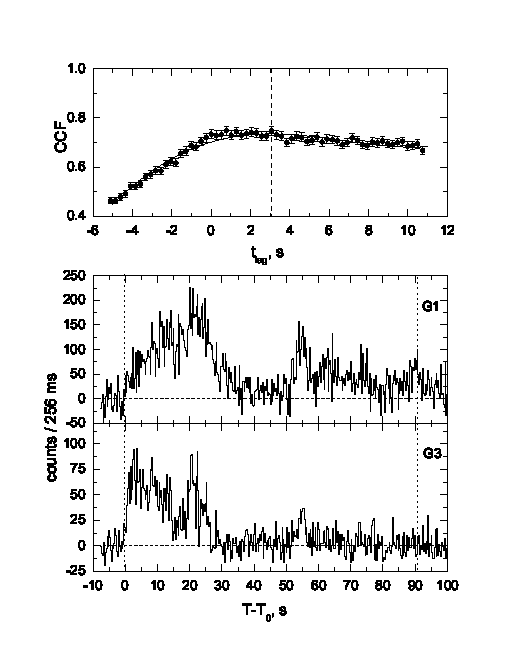
\includegraphics[width=1.0\textwidth]{id539_lag_G31.eps} \\ а)}
  \end{minipage}
  \hfill
  \begin{minipage}[h]{0.5\textwidth}
    \center{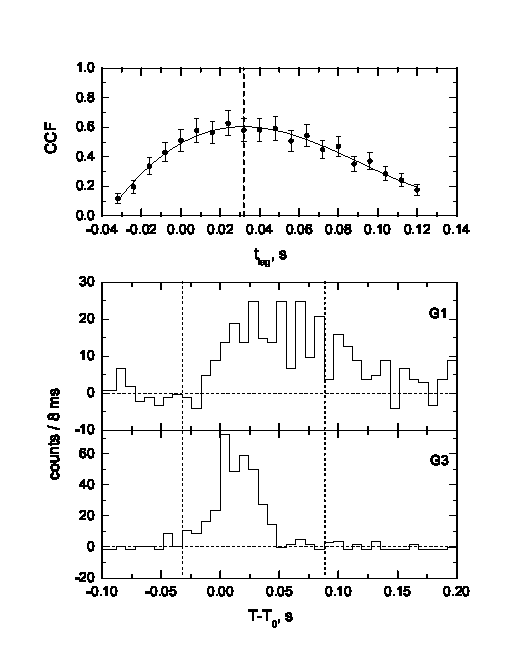
\includegraphics[width=1.0\textwidth]{id55_lag_G31.eps} \\ б)}
  \end{minipage}
  \caption{Иллюстрация вычисления лага между каналами G3 и G1 для 
  длинного GRB~970828~(а) и короткого GRB~950211~(б). 
  Вертикальные линии на нижней панели~--- границы интервала кросс-корреляции. 
  Непрерывная линия на верхней панели -- аппроксимация ККФ. Вертикальная линия 
  на верхней панели~--- значение лага на данной итерации (3.06~с и 0.03~с соответственно).}
  \label{img:lagExample}  
\end{figure}

\subsection{Aнализ спектральнх задерек}
Значения $\tau_{lag}$ между каналами G3 и G1 вычислены для 539 GRBs (505 lGRBs + 34 sGRBs) 
из них 523 всплеска имеют S/N~$\ge 10$. Значения $\tau_{lag}$ (G2-G1) вычислены 
для 1010 GRBs (954 lGRBs  + 56 sGRBs) из них 790 всплесков имеют $\rmn{S/N} \ge 10$. 
$\tau_{\rmn{lag}}$ (G3-G2) вычислены для 1010 GRBs (688 lGRBs + 148 sGRBs) 
из них 836 всплесков имеют $\rmn{S/N} \ge 10$.

Помимо обычной спектральной задержки $\tau_{\rmn{lag}}$ мы рассмотрели величину 
$\tau_{\rmn{lag}} / T_{50}$, схожая величина была рассмотрена в~\citep{Ripa_2012}. 
Преимущества этой величины в том, что она изменяется в диапазоне $\sim$~[-1;~1] и 
не зависит от красного смещения источника.  Распределения всплесков по указанным 
параметрам приведены на рис.~\ref{img:LagDistrs} и~\ref{img:NormLagDistrs}. 
Результаты применения критерия Колмогорова-Смирнова (KS) к распределениям 
$\tau_{\rmn{lag}}$ и $\tau_{\rmn{lag}} / T_{50}$ для коротких и длинных всплесков 
приведены в таблице~\ref{tab:LagDist}. Для задержек между тремя парами каналов 
$P_{KS}$ свидетельствует о том, что распределения по $\tau_{\rmn{lag}}$ 
и $\tau_{\rmn{lag}} / T_{50}$  для двух групп всплесков существенно различны. 

\subsection{Спектральные задержки коротких всплесков}
Для распределения коротких всплесков по $\tau_{\rmn{lag}}$ (G3-G1) $1\sigma$ 
интервал $\overline{\tau_{\rmn{lag}}}\pm s$, где $s$~--- стандартное отклонение, 
ограничен сверху значением $\tau_{lag}=80$~мс. $\tau_{\rmn{lag}} > 80$~мс  имеют четыре всплеска. 
Из них 3 лежат на границе кластеров коротких/жестких и длинных/мягких всплесков 
($0.5<I_{\rmn{long/soft}}<0.9$) и для одного всплеска $I_{\rmn{short/hard}}>0.5$, 
где $I$~--- индикаторная функция класса из раздела~\ref{sec:Hardness}. 
Всплеск с самой большой отрицательной задержкой $\tau_{\rmn{lag}}=-100$~мс содержит три 
импульса с последовательно нарастающей жесткостью. 

Для $\tau_{\rmn{lag}}$~(G2-G1) 1$\sigma$ интервал ограничен сверху значением $\tau_{\rmn{lag}}=60$~мс. 
$\tau_{\rmn{lag}} > 60$~мс  имеют 6 всплесков. Из них 5 имеют $I_{\rmn{long/soft}}>0.9$, 
один всплеск лежит на границе кластеров. У всех перечисленных всплесков кроме 
одного почти нет отсчётов в G3, поэтому $\tau_{\rmn{lag}}$~(G3-G1) для этих всплесков 
вычислить не удалось. Среди 5-и всплесков с существенным отрицательным лагом 
$\tau_{\rmn{lag}} <-20$~мс примерно поровну всплесков разных типов: 
два длинных/мягких всплеска и три коротких/жестких.

Для $\tau_{\rmn{lag}}$~(G3-G2) 1$\sigma$ интервал составляет [-30;~30]~мс. 
Вне этого интервала лежит 22 всплеска: 9 с $\tau_{lag} \leq -30$~мс и 13 с $\tau_{lag} \geq 30$~мс. 
Из 13 sGRB с $\tau_{lag} \geq 30$~мс четыре всплеска имеют  $\tau_{lag} \geq 60$~мс (2$\sigma$). 
Из них 3 имеют значительные остальные $\tau_{lag}$ и были отнесены к длинным/мягким всплескам, 
один всплеск является коротким/жестким.

Среди коротких всплесков с продлённым излучением 2 события имеют существенные 
спектральные задержки начального импульса \textbf{(ID=554, 1531)} и были 
классифицированы как длинные/мягкие в предыдущем разделе. Таким образом, 
можно заключить, что значительная спектральная задержка подкрепляет классификацию 
на основе распределения на плоскости жесткость-длительность.

\begin{table} [h]
 \centering
 \caption{Параметры распределений $\tau_{\rmn{lag}}$ and $\tau_{\rmn{lag}}/T_{50}$ 
 длинных и коротких всплесков}\label{tab:LagDist}
\scriptsize
%\rotate
  \begin{center}
  \begin{tabular}{c c c c c c c c c c}
  \hline
  \hline
параметр & каналы & $D_\rmn{KS}$ &  $P_\rmn{KS}$ 
&  \multicolumn{2}{c}{sGRBs} & \multicolumn{2}{c}{lGRBs} & \multicolumn{2}{c}{N ($\tau_\rmn{lag}<0$) /N$_\rmn{tot}$ }   \\
         &        &          &           
& среднее &  дисперсия   &  среднее &  дисперсия  & sGRBs & lGRBs \\
\hline
$\tau_\rmn{lag}$ (с)    & G3-G1 &	0.678 &	8.5e-14 &	0.02 &	0.06 &	0.48 &	0.74 &	0.41     & 0.14\\
$\tau_\rmn{lag}/T_{50}$ &	    &   0.297 & 5.5e-03	&   0.15 &	0.56 &	0.08 & 	0.15 &	$\cdots$ & $\cdots$    \\
$\tau_\rmn{lag}$ (с)    & G2-G1 &   0.566 &	1.1e-15	&   0.02 &	0.04 &	0.27 &	0.53 &	0.30     & 0.19 \\
$\tau_\rmn{lag}/T_{50}$ & 	    &   0.245 &	2.7e-03	&   0.04 &	0.21 &	0.04 &	0.10 &	$\cdots$ & $\cdots$	\\	
$\tau_\rmn{lag}$ (с)    & G3-G2 &	0.568 & 2.2e-35	&   0.00 &	0.03 &	0.16 &	0.88 &	0.45     & 0.27 \\
$\tau_\rmn{lag}/T_{50}$ &       &	0.307 & 1.3e-10	&   0.00 &	0.14 &	0.02 &	0.06 &	$\cdots$ & $\cdots$ \\
\hline
\end{tabular}
\end{center}
\end{table}

\begin{figure}[h]
  \begin{minipage}[h]{0.5\textwidth}
    \center{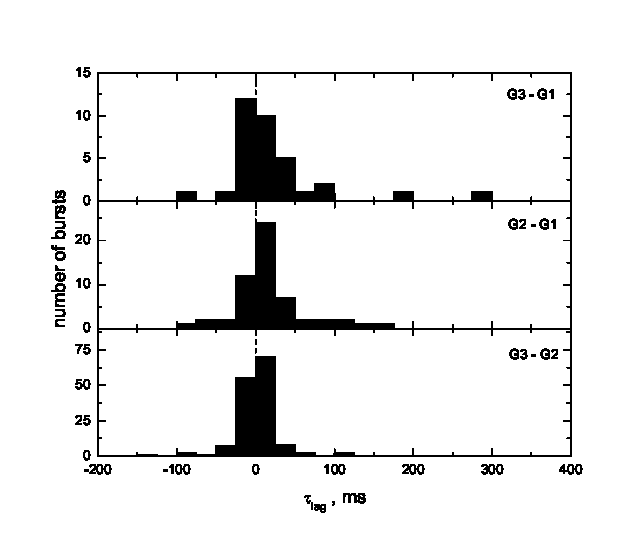
\includegraphics[width=1.0\textwidth]{gDistSGRBs} \\ а)}
  \end{minipage}
  \hfill
  \begin{minipage}[h]{0.5\textwidth}
    \center{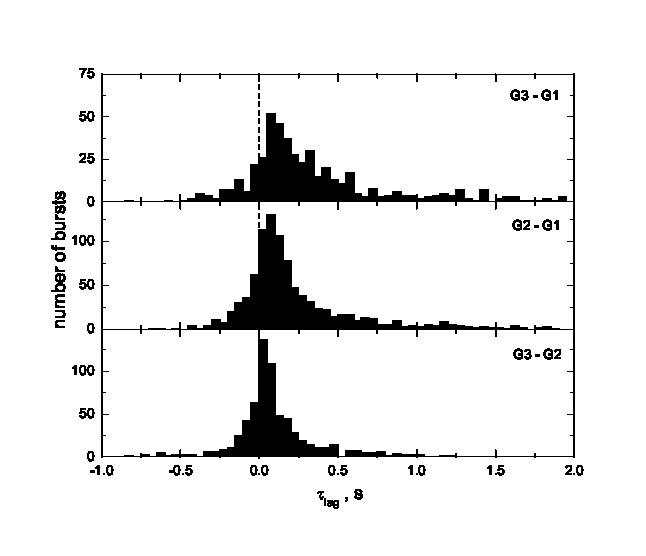
\includegraphics[width=1.0\textwidth]{gDistLGRBs} \\ б)}
  \end{minipage}
  \caption{Распределение коротких (а) и длинных (б) всплесков по спектральной задержке.}
  \label{img:LagDistrs}  
\end{figure}

\begin{figure} [h] 
  \center
  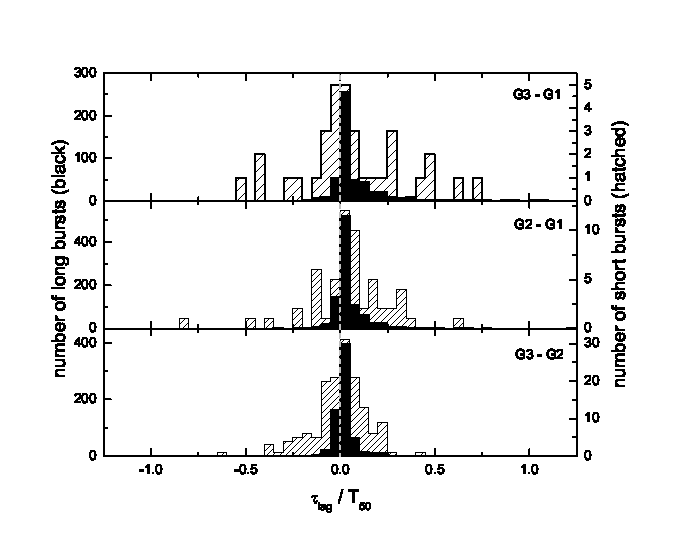
\includegraphics [width=0.8\textwidth] {DistNormLags_en}
  \caption{Распределение коротких (штрихованная гистограмма) и длинных (заполненная гистограмма)  
  всплесков по спектральной задержке, нормированной на длительность $T_{50}$.} 
  \label{img:NormLagDistrs}  
\end{figure}

\clearpage

\section{Сравнение классификаций на физические типы I и II всплесков Конус-Винд 
с определенными красными смещениями}\label{sec:Phis_Classification}
Набор всплесков Конус-Винд, зарегистрированных с ноября 1994 по декабрь 2010~г, 
содержит 87 гамма-всплесков с измеренными красными смещениями~\citep{Tsvetkova_KW_GRBs_with_z}. 
Из них три имеют сбои во временной истории: GRB~061222, GRB~081203A и GRB~090424. 
В этом разделе рассматривается набор~84~GRBs.

Этот набор содержит 8 коротких и 76 длинных GRBs. Среднее и дисперсия красных 
смещений коротких всплесков составляют~0.6 и 0.2, соответственно, для длинных 
всплесков 1.5 и 1.0, соответственно.

В работах~\citet{Zhang_2009, Kann_2010ApJ, Kann_2011ApJ} приведены классификации на 
физические типы~I и~II для 56-и всплесков, зарегистрированных Конус-Винд, из них 
8 всплесков классифицированы как Тип~I и 48 как Тип~II. 

Из 8 всплесков Типа~I, 7 относятся к кластеру коротких/жестких всплесков. 
Длинный всплеск GRB~060614 относят к коротким всплескам с продлённым излучением~\citep{Gehrels_2006_Nature}. 
Однако по нашим данным его нельзя отнести к этому классу всплесков, так как длительность 
его начального импульса $T_{50} = 2.7\pm 0.3$~с, и полная длительности $T_{50} = 49 \pm 5$~с.

Все 48 всплесков Типа II относятся к кластеру длинных/мягких всплесков~(рис.~\ref{img:T50HRzCorr}). 
Среди всплесков Типа~II, GRB~040924 имеет $T_{50} = 0.34\pm0.06$~c, но имеет 
значительную спектральную задержку, $120 \pm 30$~мс между каналами G2 и G1.

Оставшиеся 27 длинных всплесков с измеренным $z$ (кроме GRB~060614) 
\textbf{(=76 lGRBs (с $z$) - 48 Type~II - 1 (GRB~060614))}, вероятнее всего, 
относятся к Типу~II. Итого в нашем наборе всплесков с красным смещением 8 
\textbf{(=8 sGRBs (с $z$) - 1~(GRB~040924) + 1~(GRB~060614))} всплесков Типа~I 
и 76 Типа~II. Таким образом, в наборе Конус-Винд доля всплесков Типа~I составляет~10\%.

Мы проанализировали классификацию на основе жесткости и длительности в системе 
отсчёта источника всплеска. При этом $T_{50}$ уменьшается в $1+z$~раз, жесткость 
вычислялась в каналах, чьи границы соответствуют номинальным умноженным на $1/(1+z)$. 
Распределения в на плоскости $\log T_{50}$--$\log \mbox{HR}_{32}$ представлены на 
рис.~\ref{img:T50HRzCorr}.  Мы сравнили распределения по жесткостям длинных и 
коротких всплесков в системе наблюдателя и собственной системе с использованием 
критерия Колмогорова-Смирнова. Вероятность того, что жесткости всех 84-х всплесков 
являются выборкой из общего распределения в случае системы наблюдателя, 
равна 0.3\% и 3\% для системы источника.  

Также в качестве величины, характеризующей жесткость всплеска, была рассмотрена 
пиковая энергия спектра $E F_E$ -- $E_{\rmn{p}}$, полученная фитированием многоканального 
спектра моделью GRBM (Band function). $E_{\rmn{p}}$ была вычислена для 6 из 8 коротких 
всплесков и 65 из 76 длинных всплесков~\citep{Tsvetkova_KW_GRBs_with_z}. На рис.~\ref{img:T50EpzCorr} 
приведены распределения 71 всплеска на плоскости $T_{50}$--$E_{\rmn{p}}$. В собственной системе 
отсчёта только один из 6 коротких всплесков имеет $E_p > 1$~Мэв, когда среди длинных 
всплесков 16 из 67 имеют $E_{\rmn{p}} > 1$~Мэв. На основании сопоставления жесткостей 
и пиковых энергий можно заключить, что в собственной системе отсчёта 
различие в жесткостях коротких и длинных всплесков менее значимое. Наблюдаемое 
различие связано с тем, что длинные всплески, в среднем, наблюдаются на больших 
расстояниях. Наблюдаемое отсутствие коротких всплесков с измеренным $z$ 
и $E_{\rmn{p}} <400$~кэВ можно объяснить эффектом селекции триггерного алгоритма Конус-Винд. 

\begin{figure}[h]
  \begin{minipage}[h]{0.5\textwidth}
    \center{\includegraphics[width=1.0\textwidth]{logHRvslogT50z} \\ а)}
  \end{minipage}
  \hfill
  \begin{minipage}[h]{0.5\textwidth}
    \center{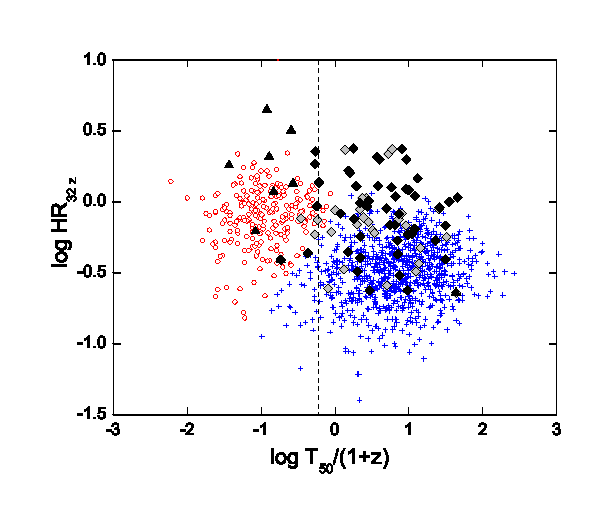
\includegraphics[width=1.0\textwidth]{logHRvslogT50zCorr} \\ б)}
  \end{minipage}
  \caption{Распределение всплесков на плоскости $\log T_{50}$--$\log \rmn{HR}_{32}$ 
  непоправленное~(а) и поправленное~(б) на космологическое красное смещение. 
  Круги~--- короткие/жесткие всплески, кресты~--- длинные/мягкие всплески. 
  Треугольники~--- короткие всплески с измеренным красным смещением, 
  заполненные треугольники~--- всплески Типа~I, ромбы~--- длинные всплески с 
  измеренным красным смещением, заполненные ромбы~--- всплески Типа~II.}
  \label{img:T50HRzCorr}  
\end{figure}

\begin{figure}[h]
  \begin{minipage}[h]{0.5\textwidth}
    \center{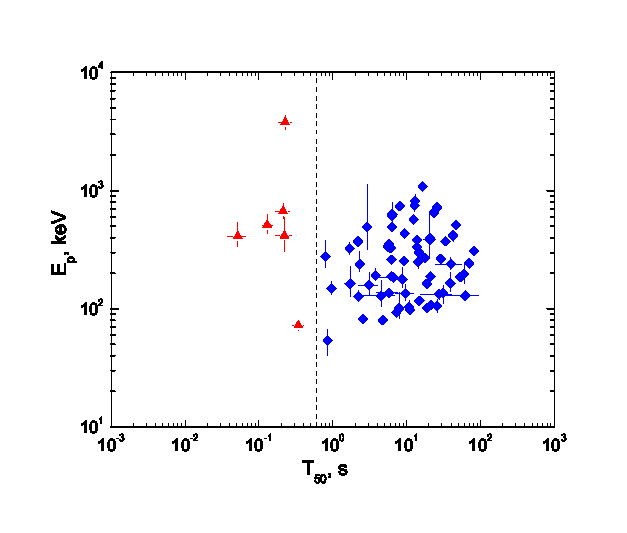
\includegraphics[width=1.0\textwidth]{EpvsT50zNcorr.eps} \\ а)}
  \end{minipage}
  \hfill
  \begin{minipage}[h]{0.5\textwidth}
    \center{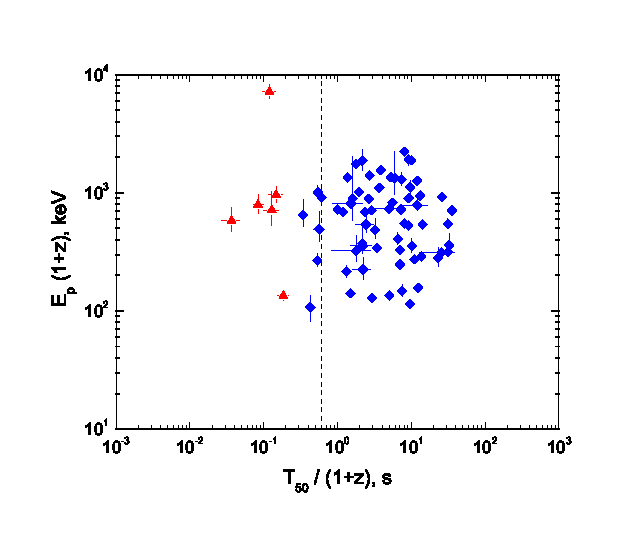
\includegraphics[width=1.0\textwidth]{EpvsT50zcorr.eps} \\ б)}
  \end{minipage}
  \caption{Распределение всплесков на плоскости $T_{50}$--$E_{\rmn{p}}$ непоправленное~(а) 
  и поправленное~(б) на космологическое красное смещение. 
  Треугольники~--- короткие всплески, ромбы~--- длинные всплески.}
  \label{img:T50EpzCorr}  
\end{figure}
\clearpage

\section{Заключение} \label{sec:Conclision}
Для набора 1834 всплесков мы вычислили длительности $T_{50}$ и $T_{90}$, жесткости, 
пиковые скорости счёта и спектральные задержки. Мы показали, что распределения 
всплесков по $T_{50}$ и $T_{90}$ хорошо аппроксимируются двумя логнормальными 
распределениями. Мы обнаружили, что параметры аппроксимации распределения $T_{50}$ 
более устойчивы к выбору порога поиска начала и конца всплеска, поэтому длительность 
$T_{50}$ более предпочтительна для классификации всплесков. В качестве границы между 
длинными и короткими всплесками мы выбрали точку пересечения логнормальных компонент 
для порога значимости $5\sigma$, $T_{50} = 0.6$~с. 

Набор коротких всплесков без продлённого излучения составляет 273 события, 
что составляет 15\% от общего числа проанализированных всплесков. Для сравнения, 
доля коротких ($T_{90}<2$~с) всплесков в каталоге BATSE равна 24\%~\citep{Meegan_2001}~\textbf{(=500/2014)}, 
в каталоге \textit{Fermi}-GBM 18\%~\citep{Paciesas_2012}, 
в каталоге \textit{Swift}-BAT 8\%~\citep{Sakamoto_2011ApJS}. 
Доля коротких всплесков, оцененная из площадей гауссовых компонент 
распределения $T_{50}$, равна 30\%. Соответствующая доля у BATSE равна 32\%~\citep{Horvath_2002} 
и 8\% у \textit{Swift}-BAT~\citep{Horvath_2008}.  

Также было обнаружено 23 всплеска, которые можно классифицировать как короткие 
всплески с продлённым излучением. Таким образом, доля всплесков с продлённым 
излучением среди коротких всплесков составляет 9\%. Соответствующая доля 
у \textit{Swift}-BAT равна 20\%~\citep{Sakamoto_2011ApJS}. 
%Подробное обсуждение коротких всплесков с продлённым излучением, обнаруженных 
%в данных Конус-Винд будет представлено в последующей публикации~\citep{Svinkin_sGRB_EE}.

Аппроксимация распределения всплесков на плоскости $\log T_{50}$--$\log \rmn{HR}_{32}$ 
набором гауссовых компонент показала наличие 2-х классов всплесков, коротких/жестких 
и длинных/мягких. При этом доля коротких/жестких всплесков составляет 21\%. По данным 
BATSE доля коротких/жестких всплесков составляет 28\%~\citep{Horvath_2002}.  
Добавление третьей компоненты даёт значимое улучшения аппроксимации, однако эта 
компонента существенно перекрывается с  компонентой, описывающей длинные всплески. 
На основании этой аппроксимации 13\% всплесков с $T_{50} < 0.6$~с относятся к классу 
длинных/мягких всплесков. При этом к классу коротких/жестких всплесков было отнесено 
только 6 из 883-х \textbf{(=911-34+6)} всплесков с $T_{50} >0.6$~с (1\%). 
Также к классу длинных/мягких всплесков, на основании жесткости и длительности 
начальных импульсов, можно отнести 2 всплеска, классифицированных на основании формы 
временной истории как короткие всплески с продлённым излучением. 

Показано, что длинные и короткие всплески имеют существенно различные распределения 
как по спектральной задержке $\tau_{\rmn{lag}}$, так и по нормированной задержке 
$\tau_{\rmn{lag}} / T_{50}$. Подтверждено, что большинство коротких всплесков 
имеют незначительную по абсолютному значению спектральную задержку $< 80$~мс, 
однако часть мягких и достаточно длинных событий $T_{50}\sim 0.6$~с имеют 
значительные задержки $\geq 80$~мс. Эти же события на основе соотношения 
жесткость-длительность были отнесены к классу длинных/мягких всплесков. 

Два всплеска с продленным излучением также имеют задержку начального импульса $> 100$~мс. 
Скорее всего, эти всплески являются длинными и ошибочно были классифицированы 
как короткие всплески с продлённым излучением.  

Сравнение классификаций на физические типы~I и~II с классификацией на основе 
длительности жесткости и спектральной задержки подтвердило, что всплески Типа~I 
относятся к коротким/жестким всплескам с малой спектральной задержкой, а всплески 
Типа~II, в основном,~--- длинные мягкие с заметной спектральной задержкой. Сравнение 
распределений всплесков как на плоскости $\log T_{50}$--$\log \rmn{HR}_{32}$, 
так и $T_{50}$--$E_{\rmn{p}}$ в системе отсчёта наблюдателя и в собственной системе 
отсчёта показывает, что различие в жесткости коротких и длинных всплесков может 
объясняться в среднем большей удалённостью последних. Недостаток коротких мягких 
всплесков с можно объяснить наблюдательной селекцией Конус-Винд.

На основании аппроксимации распределения $\log T_{50}$--$\log \rmn{HR}_{32}$ 
для 1143 всплесков, был классифицирован набор 273 коротких всплесков. 
Помимо Типа~I ($I_{\rmn{short/hard}} \geq 0.9$) и~II ($I_{\rmn{long/soft}} \geq 0.9$), 
мы отмечали всплески с "переходным"\ типом I/II ($0.1 < I_{\rmn{short/hard}} < 0.9$). 
Мы определили, что наш набор коротких всплесков содержит 214 всплесков Типа~I, 24 всплеска Типа~II 
и 35 всплесков Типа~I/II. Мы также классифицировали начальные импульсы 23 коротких 
гамма-всплесков с продлённым излучением. Из них 16 были классифицированы как Тип~I, 
один~--- Тип~II и 6~--- Типа~I/II.

\clearpage